\documentclass[10pt,xcolor=svgnames]{beamer}
\usepackage{tikz}
\setbeamertemplate{navigation symbols}{}
\usetheme[pageofpages=of,                                % String used between the current page and the
                                                         % total page count.
          alternativetitlepage=true,                     % Use the fancy title page.
          titlepagelogo=imgs/logos/ull_color_vertical,   % Logo for the first page.
          watermark=imgs/logos/logoOficialUll_watermark, % Watermark used in every page.
          watermarkheight=100px,                         % Height of the watermark.
          watermarkheightmult=4,                         % The watermark image is 4 times bigger
                                                         % than watermarkheight.
          ]{Ull}
%\progressbaroptions{headline=sections,frametitle=normal, titlepage=normal}
\usepackage{thumbpdf}
\usepackage{calc}
\usepackage{ucs}
\usepackage{listings}
\usepackage[utf8x]{inputenc}
\usepackage[spanish]{babel}
\usepackage{graphicx}
\usepackage{pgf,pgfarrows,pgfnodes,pgfautomata,pgfheaps,pgfshade}
\usepackage{pgfpages}
\usepackage{xxcolor}
\usetikzlibrary{arrows}
\usetikzlibrary{trees}
\pdfinfo
{
  /Title       (CSUOptimizer: Optimización de apuntados en el proyecto EMIR)
  /Creator     (Pedro Hdez. Martín)
  /Author      (Pedro Hdez. Martín)
  /Subject     (PFC-EMIR, 16 Jul 2013)
}
%%%%%%%%%%%%%%%%%%%%%%%%%%%%%%%%%%%%%%%%%%%%%%%%%%%%%%%%%%%%%%%%%%%%%%%%%%%%%%%%%%%%%%%%%%%%
\definecolor{marron}       {rgb}{0.496, 0.203, 0.152}
\definecolor{verde-claro}  {rgb}{0.625, 0.734, 0.199}
\definecolor{oscuro}       {rgb}{0.187, 0.141, 0.285}
\definecolor{gris}     	   {rgb}{0.500, 0.500, 0.500}
\definecolor{bgd-listings} {rgb}{0.999, 0.999, 0.900}
\definecolor{gray97}{gray}{.97}
\definecolor{gray75}{gray}{.75}
\definecolor{gray45}{gray}{.45}
\lstloadlanguages{C++}
\lstset{
  language=C++,                          	% C++
	keywordstyle=\color{black}\textbf,   	% BGD: Palabras clave en negro y negrita
	%showstringspaces=false
	%backgroundcolor=\color{yellow},     	% Códigos sobre fondo amarillo
  backgroundcolor=\color{bgd-listings},
	basewidth={0.6em, 0.45em},
	%basicstyle=\small,                   	% Listados en small
	basicstyle=\scriptsize,                   	% Listados en small
	breakautoindent=true,									% BGD: Autoindentar líneas cortadas
	breaklines=true,											% BGD: Cortar líneas si son muy grandes
	captionpos=b,													% Posición de los títulos abajo (bottom)
	columns=fixed,
  %commentstyle=\color{blue},           % comentarios en azul
  %commentstyle=\color{gray45},
	commentstyle=\color{blue}\textit,  	 	% BGD: Comentarios en azul cursiva
	directivestyle=\color{oscuro}\texttt,	
	emph={hicuda,data,region,pragma,acc,loop,private,collapse,kernel,kernels,copy,copyin,llc,omp},								% BGD: Resaltar las palabras pragma, llc y omp
	emphstyle=\textbf,
	extendedchars=true,									  % BGD: Utiliza caracteres extendidos (tildes, etc.)
	firstnumber=1,												% BGD: Número línea empieza en 0 (línea vacía, no se muestra)
  %frame=lines,                        	% Línea arriba y abajo de cada listado de código
	%frame=trbl,														% BGD: Cuadro  (t/T: top, r/R: right, b/B: bottom, l/L: left): x->thin, X->thick
	framesep=4pt,
	%framexleftmargin=5mm,									% BGD: Margen izquierdo de los marcos (para que quepan num. de línea) 
  %identifierstyle=\ttfamily,
	identifierstyle=\color{black}\ttfamily, % BGD: Identificadores en negro	
	inputencoding=latin1,									
	keepspaces=true,											% BGD: Mantener espacios
	numberblanklines=false,								% BGD: No pone números de línea en líneas vacías
	numbers=left,													% BGD: Números de línea a la izquierda
	numbersep=8pt,												% BGD: Números de línea separados 8 pts a la izquierda
	postbreak=\space,					  					% BGD: Cortar líneas por espacios
	rulesepcolor=\color{black},						% BGD: Color de los cuadros azul
	showstringspaces=false,								% BGD: No mostar espacios
	stepnumber=1,													% BGD: Números línea a línea
	tabsize=2,														% BGD: Tamaño de tabulador para indentaciones = 2
  %framerule=0pt,
  %keywordstyle=\color{red},            % Palabras clave en rojo
  keywordstyle=\bfseries,
	%stringstyle=\color{red}\texttt,       % BGD: Cadenas en rojo
  %stringstyle=\color{green},           % cadenas en verde
  stringstyle=\ttfamily,
}

\title{\textbf{\texttt{CSUOptimizer}: Optimización de apuntados en el proyecto EMIR}}
\author[Hernández Martín]{%
  \textbf{Pedro Orlando~Hernández Martín}}
\institute[Universidad de La Laguna]{
}
%\date[HAC-2012]{\textbf{HAC-2012, Leganés, July 13}}
\date[PFC-2013]{\textsc{Proyecto de Fin de Carrera,\\
                        Ingeniería Informática} \\
                        La Laguna, 16 Julio 2013}
\subject{PFC - EMIR}

%\AtBeginSection[]
%{
%  \frame<handout:0>
%  {
%    \frametitle{Índice}
%    \tableofcontents[current]
%  }
%}

\begin{document}
\newcommand{\CSUO}{\texttt{CSUOptimizer}{}}          

\frame{\titlepage}
%\section{Introducción}

%%%%%%%%%%%%%%%%%%%%%%%%%%%%%%%%%%%%%%%%%%%%%%%%%%%%%%%%%%%%%%
\begin{frame}
    \frametitle{Instituto de Astrofísica de Canarias}
    \block{IAC}
    \endblock{}
		\begin{center}
    
\includegraphics[width=0.5\linewidth]{FIGURES/logoIAC}
		\end{center}
\end{frame}
%%%%%%%%%%%%%%%%%%%%%%%%%%%%%%%%%%%%%%%%%%%%%%%%%%%%%%%%%%%%%%

%%%%%%%%%%%%%%%%%%%%%%%%%%%%%%%%%%%%%%%%%%%%%%%%%%%%%%%%%%%%%%
\begin{frame}
    \frametitle{Instituto de Astrofísica de Canarias}
    \block{Sedes}
    \endblock{}
		\begin{center}
    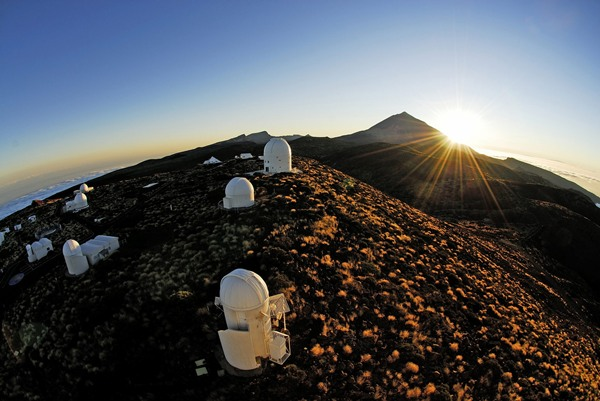
\includegraphics[width=0.7\linewidth]{FIGURES/IAC}
		\end{center}
\end{frame}
%%%%%%%%%%%%%%%%%%%%%%%%%%%%%%%%%%%%%%%%%%%%%%%%%%%%%%%%%%%%%%

%%%%%%%%%%%%%%%%%%%%%%%%%%%%%%%%%%%%%%%%%%%%%%%%%%%%%%%%%%%%%%
\begin{frame}
    \frametitle{Gran Telescopio Canarias}
    \block{GTC}
    \endblock{}
		\begin{center}
    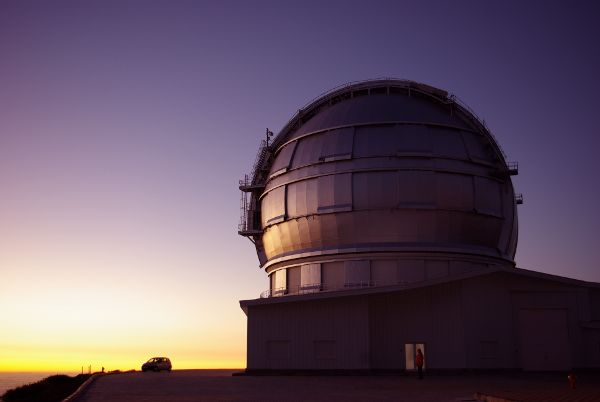
\includegraphics[width=0.8\linewidth]{FIGURES/GTC}
		\end{center}
\end{frame}
%%%%%%%%%%%%%%%%%%%%%%%%%%%%%%%%%%%%%%%%%%%%%%%%%%%%%%%%%%%%%%

%%%%%%%%%%%%%%%%%%%%%%%%%%%%%%%%%%%%%%%%%%%%%%%%%%%%%%%%%%%%%%
\begin{frame}
    \frametitle{Proyecto GOYA}
    \centering{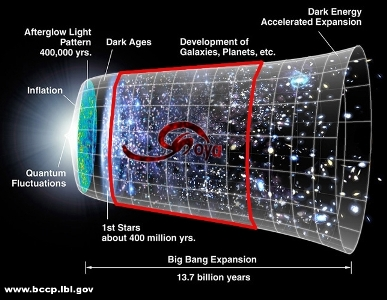
\includegraphics[width=0.4\linewidth]{FIGURES/goya}}
    \block{GOYA: Galaxy Origins and Young Assembly}
    \begin{itemize}
		\item Objetivo: entender cómo se forman y evolucionan las galaxias observando sus propiedades en una época de máximo crecimiento
		\item Investiga las propiedades de las galaxias más lejanas
		\item A distancias de 8000--13000 millones de años luz
		\item Llevará a cabo la primera exploración sistemática de la población de galaxias poco después del nacimiento del universo
    \end{itemize}
    \endblock{}
\end{frame}
%%%%%%%%%%%%%%%%%%%%%%%%%%%%%%%%%%%%%%%%%%%%%%%%%%%%%%%%%%%%%%

%%%%%%%%%%%%%%%%%%%%%%%%%%%%%%%%%%%%%%%%%%%%%%%%%%%%%%%%%%%%%%
\begin{frame}
    \frametitle{El Proyecto EMIR}
    \centering{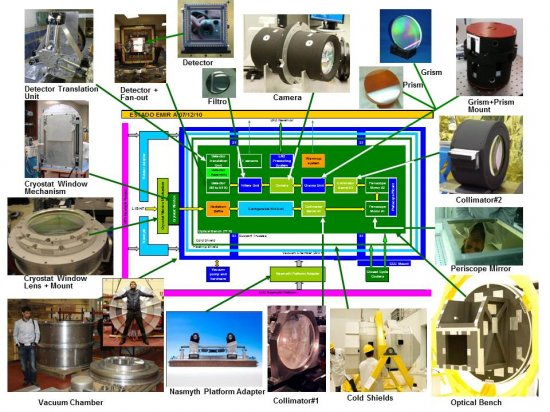
\includegraphics[width=0.7\linewidth]{FIGURES/emir}}
    %\centering{
\includegraphics[width=0.6\linewidth]{FIGURES/logoEMIR}}
    \block{EMIR: Espectrógrafo Multiobjeto Infrarrojo}
		EMIR es un cámara de gran campo y espectrógrafo de resolución intermedia en el infrarrojo cercano para el telescopio GTC
    \endblock{}
\end{frame}
%%%%%%%%%%%%%%%%%%%%%%%%%%%%%%%%%%%%%%%%%%%%%%%%%%%%%%%%%%%%%%

%\begin{frame}{Índice}
% \begin{columns}[t]
%		\column{.5\linewidth}
%		  \alert<1>{\small{\tableofcontents[sections={1}]}}
%		  \vspace{5mm}
%		  \alert<2>{\small{\tableofcontents[sections={2}]}}
%		  \vspace{5mm}
%		  \alert<3>{\small{\tableofcontents[sections={3}]}}
%		  \vspace{5mm}
%      \alert<4>{\small{\tableofcontents[sections={4}]}}
%		  \vspace{5mm}
% \end{columns}
%\end{frame}


%%%%%%%%%%%%%%%%%%%%%%%%%%%%%%%%%%%%%%%%%%%%%%%%%%%%%%%%%%%%%
%%%%%%%%%%%%%%%%%%%%%%%%%%%%%%%%%%%%%%%%%%%%%%%%%%%%%%%%%%%%%
%%%%%%%%%%%%%%%%%%%%%%%%%%%%%%%%%%%%%%%%%%%%%%%%%%%%%%%%%%%%%

%\AtBeginSection[]
%{
%   \begin{frame}
%       \frametitle{Índice}
%       \footnotesize{
%         \tableofcontents[currentsection,hideothersubsections]
%       }
%   \end{frame}
%}
%


\AtBeginSection[]
{
  \frame<handout:0>
  {
    \frametitle{Índice}
    \tableofcontents[current]
  }
}
%%%%%%%%%%%%%%%%%%%%%%%%%%%%%%%%%%%%%%%%%%%%%%%%%%%%%%%%%
\frame{\frametitle{Índice}\tableofcontents}
\section{Introducción}
\section{Unidad de rejillas configurable}
	  %\section{CSU de EMIR}

%%%%%%%%%%%%%%%%%%%%%%%%%%%%%%%%%%%%%%%%%%%%%%%%%%%%%%%%%%%%%%
\begin{frame}
    \frametitle{CSU: Configurable Split Unit}
    \centering{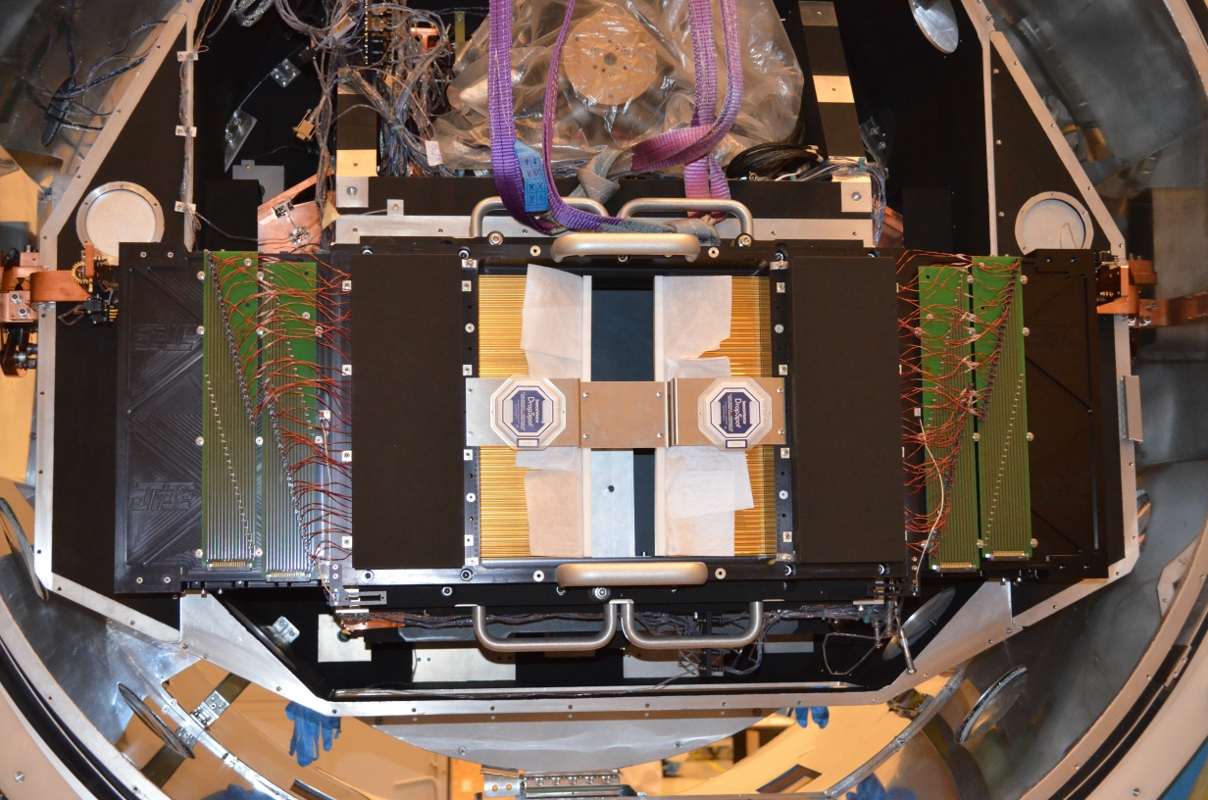
\includegraphics[width=0.8\linewidth]{FIGURES/DSC_0750}}
    \block{CSU}
    \begin{itemize}[<+->]
    \item Dimensiones $\rightarrow 240\times400$ arcosegundos
    \item 55 pares de barras
    \item Rotación
    \end{itemize}
    \endblock{}
\end{frame}
%%%%%%%%%%%%%%%%%%%%%%%%%%%%%%%%%%%%%%%%%%%%%%%%%%%%%%%%%%%%%%

%%%%%%%%%%%%%%%%%%%%%%%%%%%%%%%%%%%%%%%%%%%%%%%%%%%%%%%%%%%%%%
\begin{frame}
    \frametitle{Apuntado - Representación gráfica}
    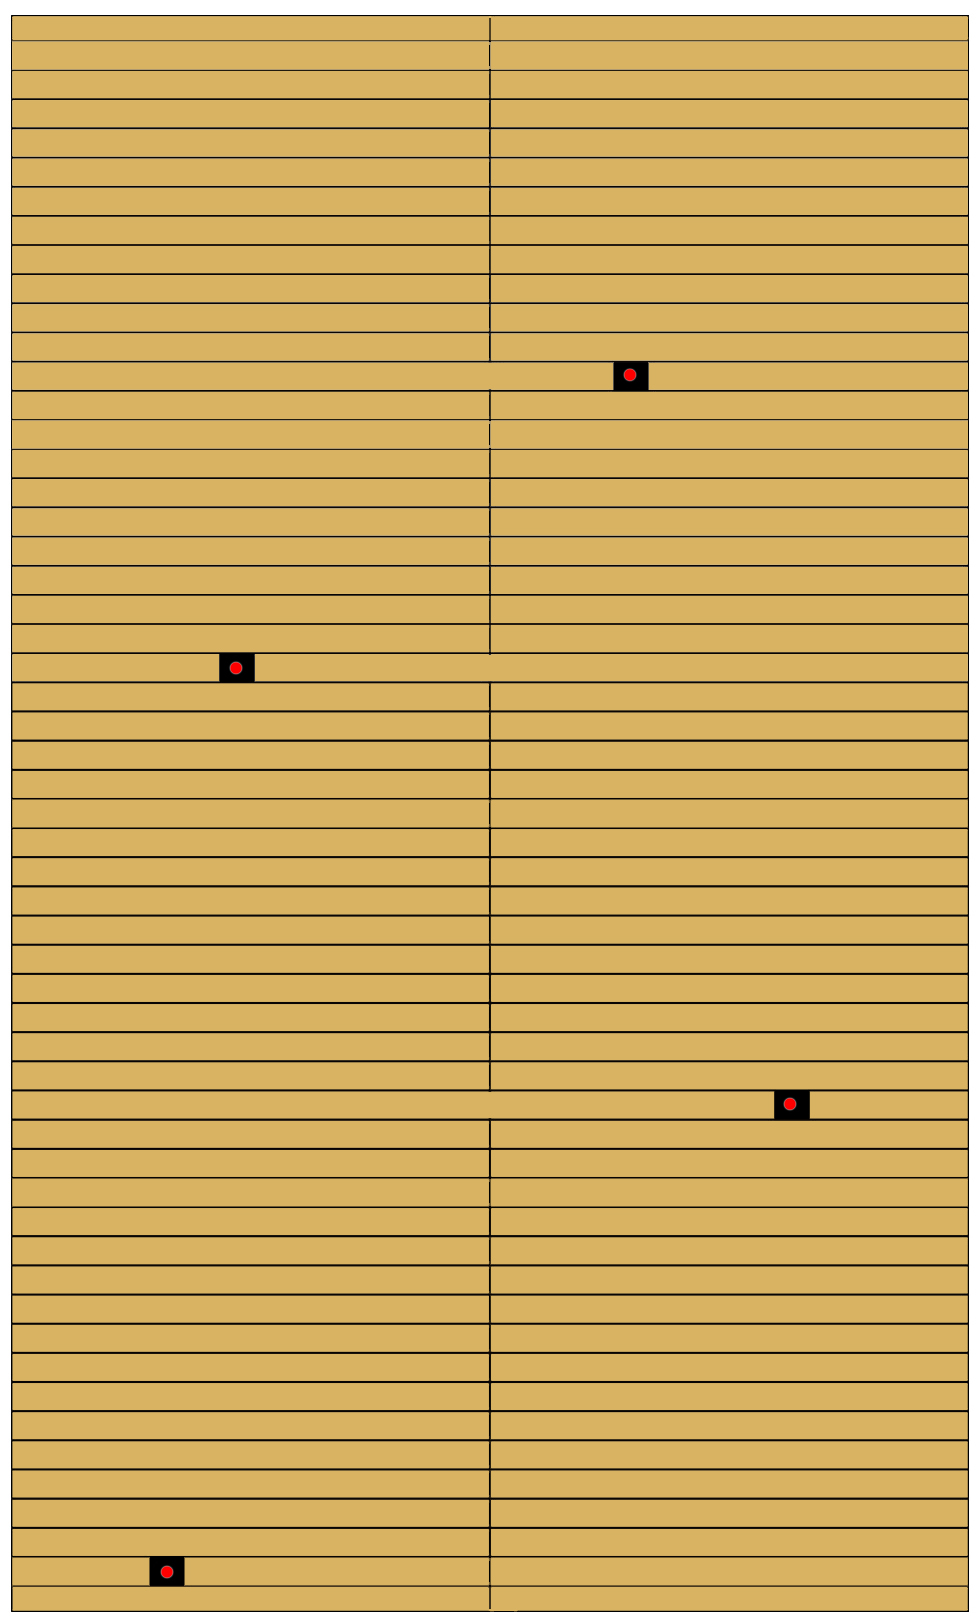
\includegraphics[height=0.8\textheight]{FIGURES/CSU-puntos}
    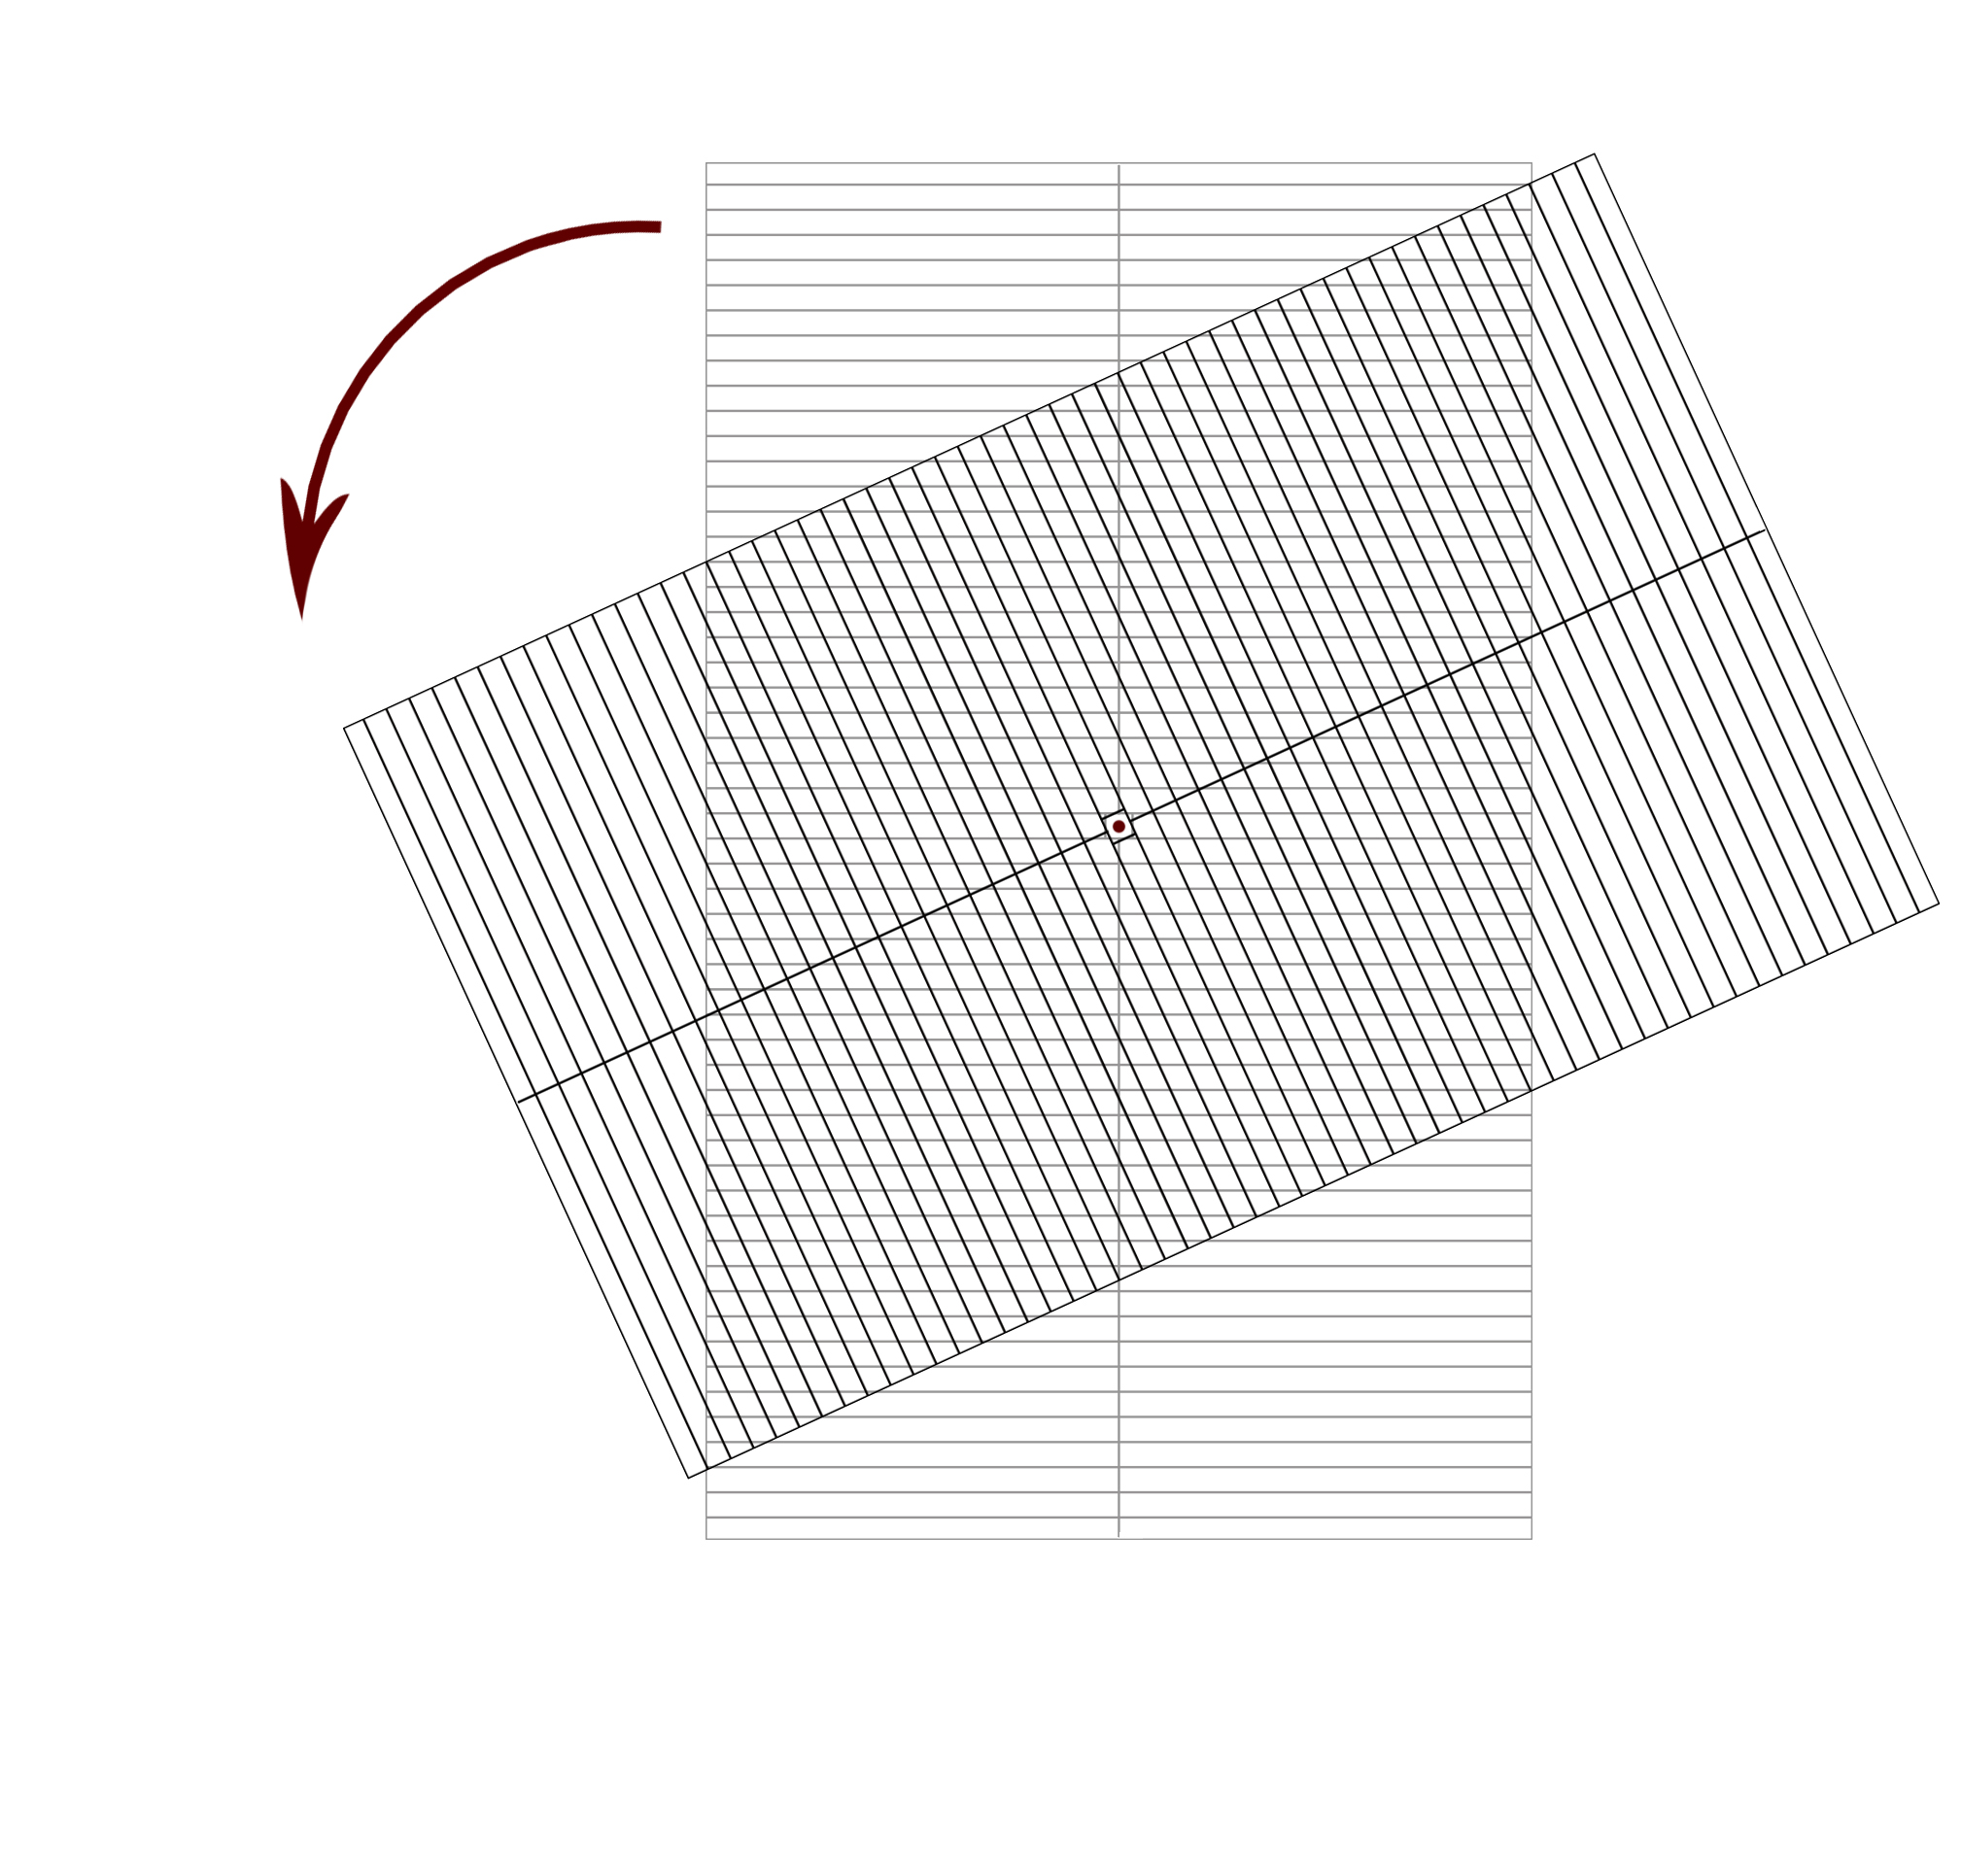
\includegraphics[width=0.7\linewidth]{FIGURES/CSU-giro}
\end{frame}
%%%%%%%%%%%%%%%%%%%%%%%%%%%%%%%%%%%%%%%%%%%%%%%%%%%%%%%%%%%%%%

%%%%%%%%%%%%%%%%%%%%%%%%%%%%%%%%%%%%%%%%%%%%%%%%%%%%%%%%%%%%%%
\begin{frame}
    \frametitle{Problema}
    \centering{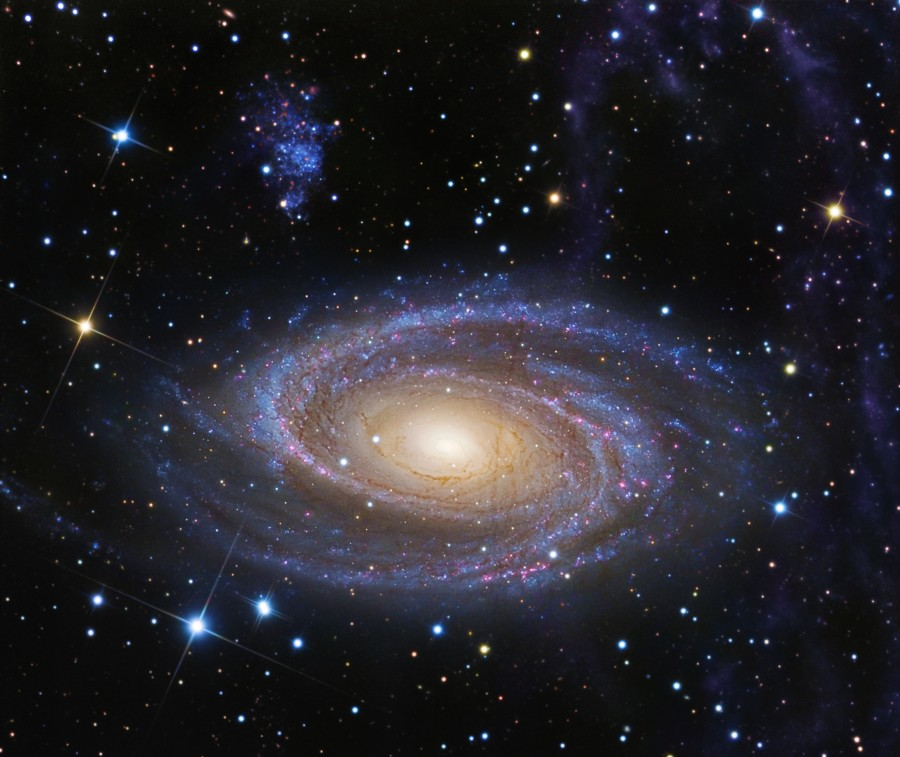
\includegraphics[width=0.6\linewidth]{FIGURES/lrg_ngc3031gabany900c}}
    \block{Descripción}
    \begin{itemize}[<+->]
		\item Número de objetos a observar $>>$ número de barras
    \item Minimizar el tiempo de observación es crítico
    \item Configuración compleja
    \end{itemize}
    \endblock{}
\end{frame}
%%%%%%%%%%%%%%%%%%%%%%%%%%%%%%%%%%%%%%%%%%%%%%%%%%%%%%%%%%%%%%

%%%%%%%%%%%%%%%%%%%%%%%%%%%%%%%%%%%%%%%%%%%%%%%%%%%%%%%%%%%%%%
\begin{frame}
    \frametitle{Objetivos}
    \block{Una aplicación que:}
      \begin{itemize}[<+->]
      \item Resuelva el problema
      \item Minimice el tiempo de respuesta
      \item Contemple prioridades
      \item Contemple Beam Switching
      \end{itemize}
    \endblock{}
\end{frame}
%%%%%%%%%%%%%%%%%%%%%%%%%%%%%%%%%%%%%%%%%%%%%%%%%%%%%%%%%%%%%%

%%%%%%%%%%%%%%%%%%%%%%%%%%%%%%%%%%%%%%%%%%%%%%%%%%%%%%%%%%%%%%
\begin{frame}
    \frametitle{Problema}
    \centering{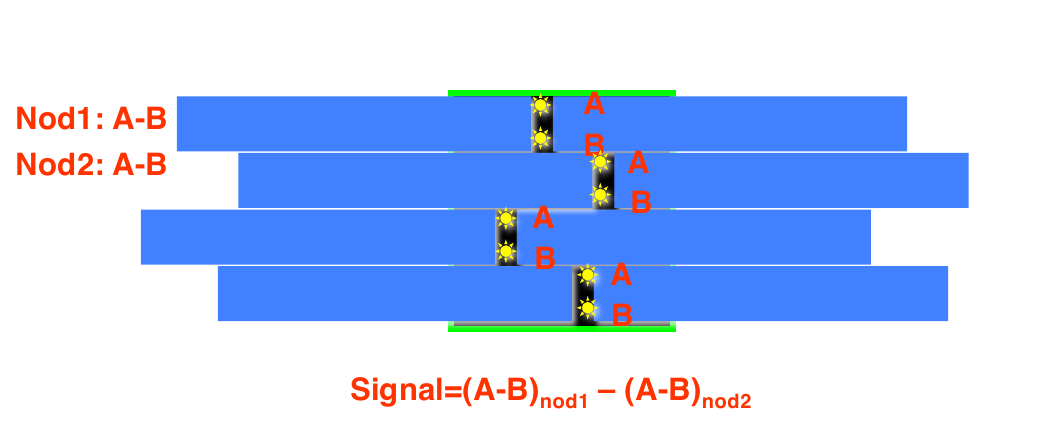
\includegraphics[width=\linewidth]{FIGURES/beamexplication}}
    \block{Beam switching}
		\begin{itemize}
		\item Método para obtener mediciones más precisas
		\item Se mide la luz procedente del objeto y la de la bóveda celeste
		\item Se mueve ligeramente la posición del medidor y se repite la medida
		\end{itemize}
    \endblock{}
\end{frame}
%%%%%%%%%%%%%%%%%%%%%%%%%%%%%%%%%%%%%%%%%%%%%%%%%%%%%%%%%%%%%%

%%%%%%%%%%%%%%%%%%%%%%%%%%%%%%%%%%%%%%%%%%%%%%%%%%%%%%%%%%%%%%
\begin{frame}
    \frametitle{Solución}
    \block{Frentes de actuación}
    \begin{itemize}
		\item Clustering
    \item Algoritmo Constructivo
    \end{itemize}
    \endblock{}
\end{frame}
%%%%%%%%%%%%%%%%%%%%%%%%%%%%%%%%%%%%%%%%%%%%%%%%%%%%%%%%%%%%%%

%%%%%%%%%%%%%%%%%%%% Code  %%%%%%%%%%%%%%%%%%%%%%%%%%%%%%%%%%%
\begin{frame}[fragile]
\frametitle{Clustering}
\block{DBScan}
\endblock{}
%\begin{algorithm}
\begin{lstlisting}[linewidth=\linewidth, mathescape,
numbers=none,basicstyle=\ttfamily\footnotesize]
DBSCAN($D$, $eps$, $MinPts$) {
   $C = 0$
   For(cada punto $P$ no visitado en el cjto de datos $D$) {
      marcar $P$ como visitado
      $NeighborPts =$ regionQuery($P$, $eps$)
      If(sizeof($NeighborPts$) $< MinPts$)
         marcar $P$ como $RUIDO$
      else {
         $C =$ siguiente cluster
         expandCluster($P$, $NeighborPts$, $C$, $eps$, $MinPts$)
      }   
   }   
}
\end{lstlisting}
%\end{algorithm}
\end{frame}
%%%%%%%%%%%%%%%%%%%%%%%%%%%%%%%%%%%%%%%%%%%%%%%%%%%%%%%%%%%%%%

%%%%%%%%%%%%%%%%%%%%%%%%%%%%%%%%%%%%%%%%%%%%%%%%%%%%%%%%%%%%%%
\begin{frame}
    \frametitle{Clustering}
    \block{DBSCAN}
    \endblock{}
		\begin{center}
    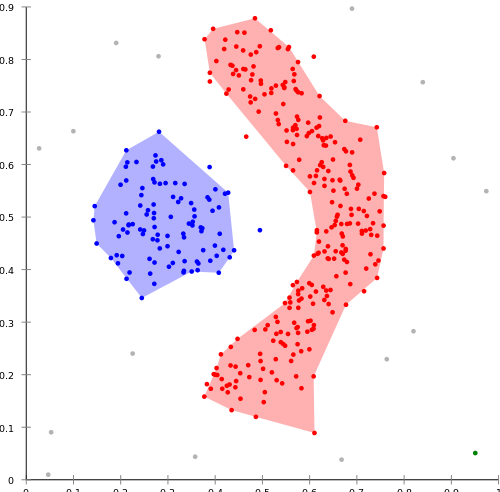
\includegraphics[height=0.8\textheight]{FIGURES/DBSCAN-density-data}
		\end{center}
\end{frame}
%%%%%%%%%%%%%%%%%%%%%%%%%%%%%%%%%%%%%%%%%%%%%%%%%%%%%%%%%%%%%%

%%%%%%%%%%%%%%%%%%%%%%%%%%%%%%%%%%%%%%%%%%%%%%%%%%%%%%%%%%%%%%
\begin{frame}
    \frametitle{Clustering}
    \block{DBSCAN}
    \endblock{}
		\begin{center}
    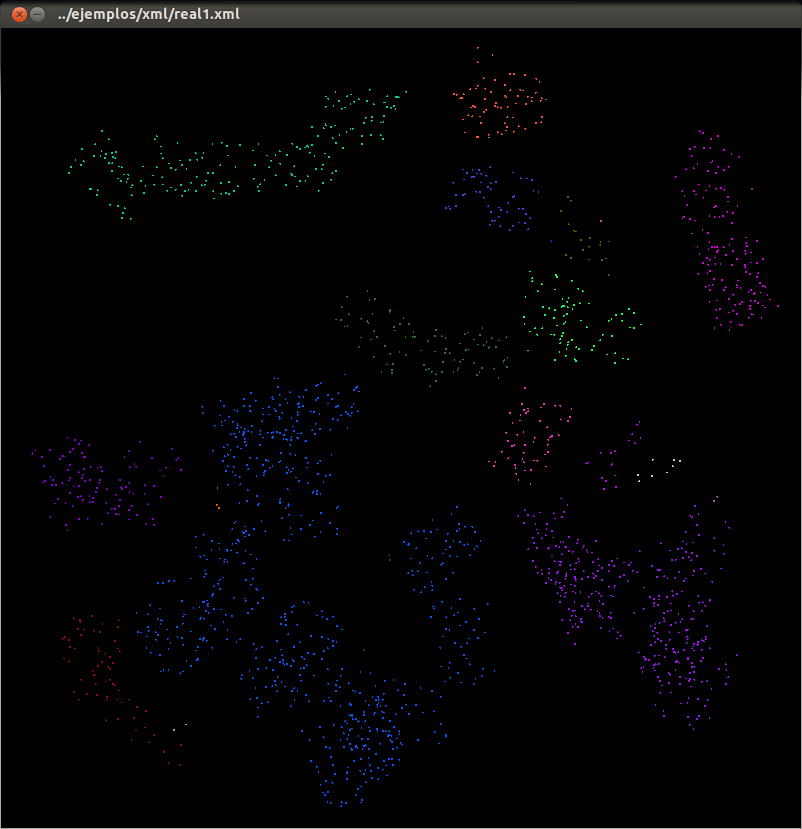
\includegraphics[height=0.8\textheight]{FIGURES/dbscan-e86-m4}
		\end{center}
\end{frame}
%%%%%%%%%%%%%%%%%%%%%%%%%%%%%%%%%%%%%%%%%%%%%%%%%%%%%%%%%%%%%%

%%%%%%%%%%%%%%%%%%%%%%%%%%%%%%%%%%%%%%%%%%%%%%%%%%%%%%%%%%%%%%
\begin{frame}[fragile]
    \frametitle{Solución}
    \block{Algoritmo Constructivo}
    \endblock{}
		\begin{center}
    \begin{lstlisting}[linewidth=\linewidth, mathescape,
    numbers=none,basicstyle=\ttfamily\footnotesize]
For (Cada tipo de ordenacion) {
  ordenar los objetos
  While (queden objetos por cubrir) {
    $p \leftarrow$ siguiente punto de la lista no eliminado
    $C =$ mejor CSU $\in$ crearApuntados($p$, $puntos$)
    puntos -= $\forall$ puntos $\in C$
    Solucion$[tipo orden]  = Solucion$[tipo orden] $\bigcup{C}$
  }
}
$Sol =$ min(Solucion[tipo orden])
    \end{lstlisting}
		\end{center}
\end{frame}
%%%%%%%%%%%%%%%%%%%%%%%%%%%%%%%%%%%%%%%%%%%%%%%%%%%%%%%%%%%%%%

%%%%%%%%%%%%%%%%%%%% Code  %%%%%%%%%%%%%%%%%%%%%%%%%%%%%%%%%%%
\begin{frame}[fragile]
    \frametitle{Algoritmo Constructivo}
    \block{Fase 1: Obtención de objetos}
    \endblock{}
    \begin{lstlisting}[linewidth=\linewidth, numbers=none,basicstyle=\ttfamily\footnotesize]
int estaDentro(const Element &p) const {
  static double new_x, new_y, zone;                            
  if (estaDentro2(p)) {
    testeo(p, new_x, new_y);
    zone = sqrt((Ax - new_x) * (Ax - new_x)i + (Ay - new_y) * (Ay - new_y));
    barra = (int)(zone / DIST_BARRAS);
    if (barra == NUM_BARRAS)
      return 0;
    rango = zone - (barra * DIST_BARRAS);
    distancia = sqrt((p.getx() - new_x) * (p.getx() - new_x) + (p.gety() - new_y) * (p.gety() - new_y));
    if (distancia > 2*ANCHO)
      return 0;
    if (barras_ocupadas[barra])
      return p_potencial(rango, barra);
  }
  return 0;
}
    \end{lstlisting}
\end{frame}
%%%%%%%%%%%%%%%%%%%%%%%%%%%%%%%%%%%%%%%%%%%%%%%%%%%%%%%%%%%%%%

%%%%%%%%%%%%%%%%%%%%%%%%%%%%%%%%%%%%%%%%%%%%%%%%%%%%%%%%%%%%%%
\begin{frame}
    \frametitle{Algoritmo Constructivo}
    \block{Fase 1: Obtención de objetos}
    \endblock{}
		\begin{center}
    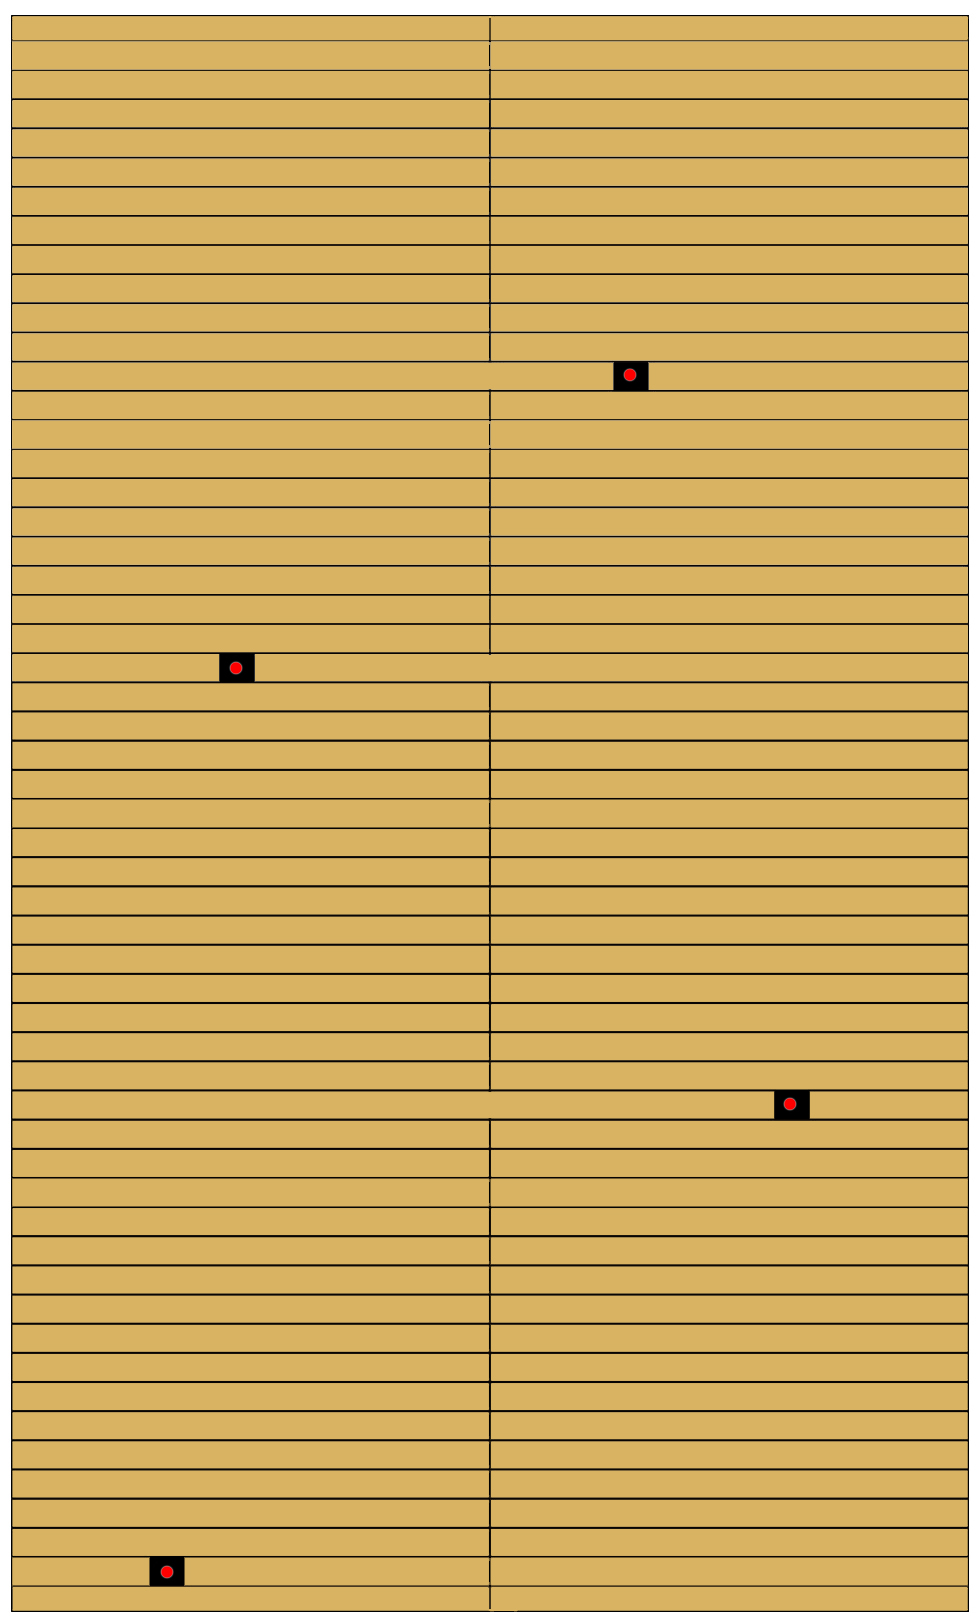
\includegraphics[height=0.8\textheight]{FIGURES/CSU-puntos}
		\end{center}
\end{frame}
%%%%%%%%%%%%%%%%%%%%%%%%%%%%%%%%%%%%%%%%%%%%%%%%%%%%%%%%%%%%%%

%%%%%%%%%%%%%%%%%%%% Code  %%%%%%%%%%%%%%%%%%%%%%%%%%%%%%%%%%%
\begin{frame}[fragile]
    \frametitle{Algoritmo Constructivo}
    \block{Fase 2: Mejora}
    \endblock{}
    \begin{lstlisting}[linewidth=\linewidth, mathescape,
    numbers=none,basicstyle=\ttfamily\footnotesize]
For(Todas las rotaciones posibles) {
    Crear $CSU$ con centro en en el objeto
    rellenar_con_puntos($CSU$, $lista\_objetos$)
    While(numero de puntos en $CSU$ cambie) {
        movimiento de mejora arriba
        rellenar_con_puntos($CSU$, $puntos$)
        movimiento de mejora abajo
        rellenar_con_puntos($CSU$, $puntos$)
        movimiento de mejora izquierda
        rellenar_con_puntos($CSU$, $puntos$)
        movimiento de mejora derecha
        rellenar_con_puntos($CSU$, $puntos$)
    }
    $posibles = posibles \bigcup{CSU}$
}
    \end{lstlisting}
\end{frame}
%%%%%%%%%%%%%%%%%%%%%%%%%%%%%%%%%%%%%%%%%%%%%%%%%%%%%%%%%%%%%%

%%%%%%%%%%%%%%%%%%%%%%%%%%%%%%%%%%%%%%%%%%%%%%%%%%%%%%%%%%%%%%
\begin{frame}
    \frametitle{Algoritmo Constructivo}
    \block{Fase 2: Mejora}
    \endblock{}
		\begin{center}
    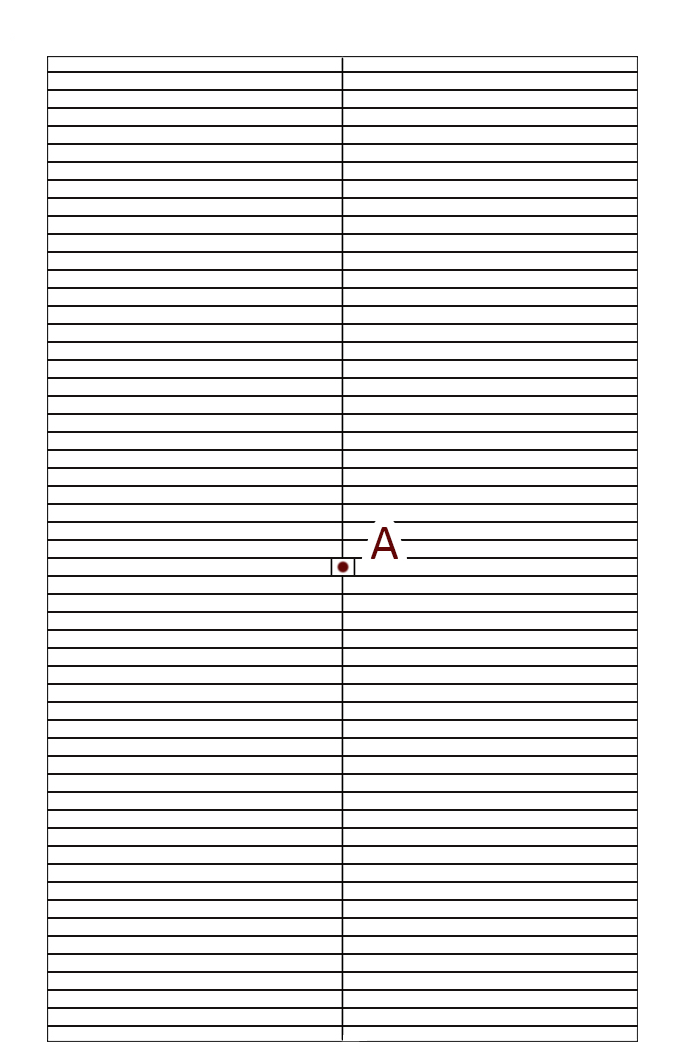
\includegraphics[height=0.8\textheight]{FIGURES/paso1}
		\end{center}
\end{frame}
%%%%%%%%%%%%%%%%%%%%%%%%%%%%%%%%%%%%%%%%%%%%%%%%%%%%%%%%%%%%%%

%%%%%%%%%%%%%%%%%%%%%%%%%%%%%%%%%%%%%%%%%%%%%%%%%%%%%%%%%%%%%%
\begin{frame}
    \frametitle{Algoritmo Constructivo}
    \block{Fase 2: Mejora}
    \endblock{}
		\begin{center}
    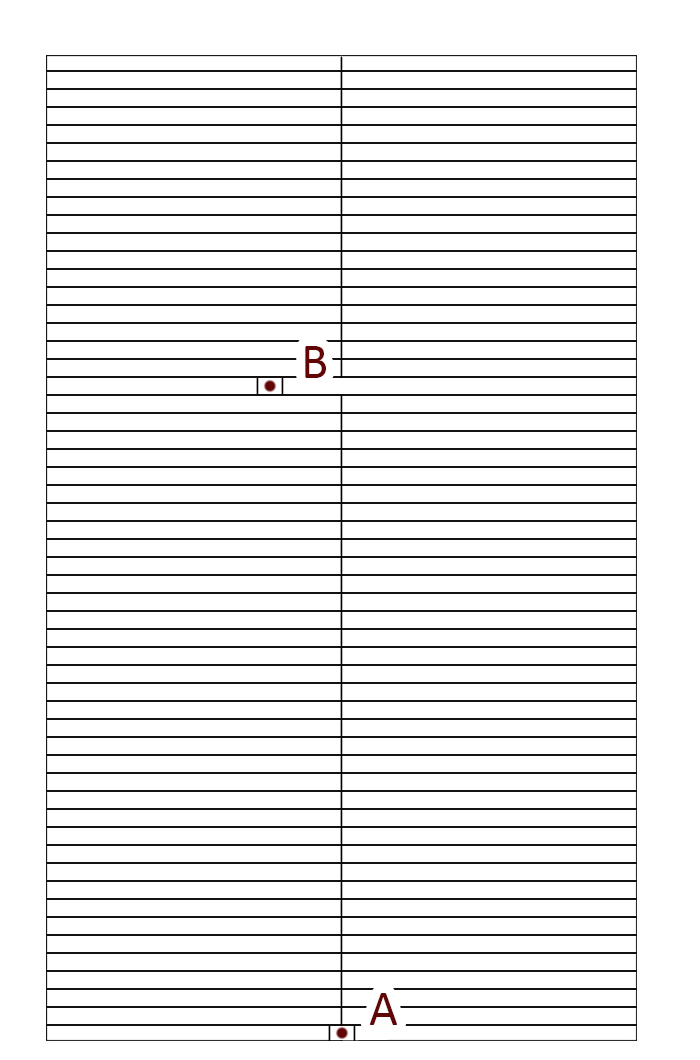
\includegraphics[height=0.8\textheight]{FIGURES/paso2}
		\end{center}
\end{frame}
%%%%%%%%%%%%%%%%%%%%%%%%%%%%%%%%%%%%%%%%%%%%%%%%%%%%%%%%%%%%%%

%%%%%%%%%%%%%%%%%%%%%%%%%%%%%%%%%%%%%%%%%%%%%%%%%%%%%%%%%%%%%%
\begin{frame}
    \frametitle{Algoritmo Constructivo}
    \block{Fase 2: Mejora}
    \endblock{}
		\begin{center}
    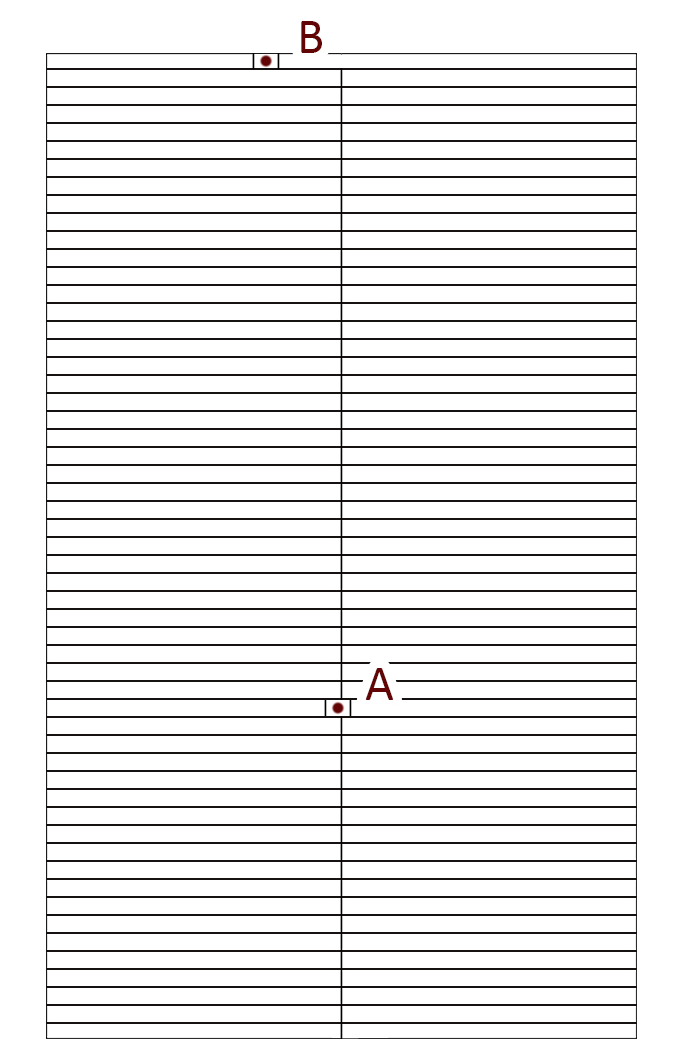
\includegraphics[height=0.8\textheight]{FIGURES/paso3}
		\end{center}
\end{frame}
%%%%%%%%%%%%%%%%%%%%%%%%%%%%%%%%%%%%%%%%%%%%%%%%%%%%%%%%%%%%%%

%%%%%%%%%%%%%%%%%%%%%%%%%%%%%%%%%%%%%%%%%%%%%%%%%%%%%%%%%%%%%%
\begin{frame}
    \frametitle{Algoritmo Constructivo}
    \block{Fase 2: Mejora}
    \endblock{}
		\begin{center}
    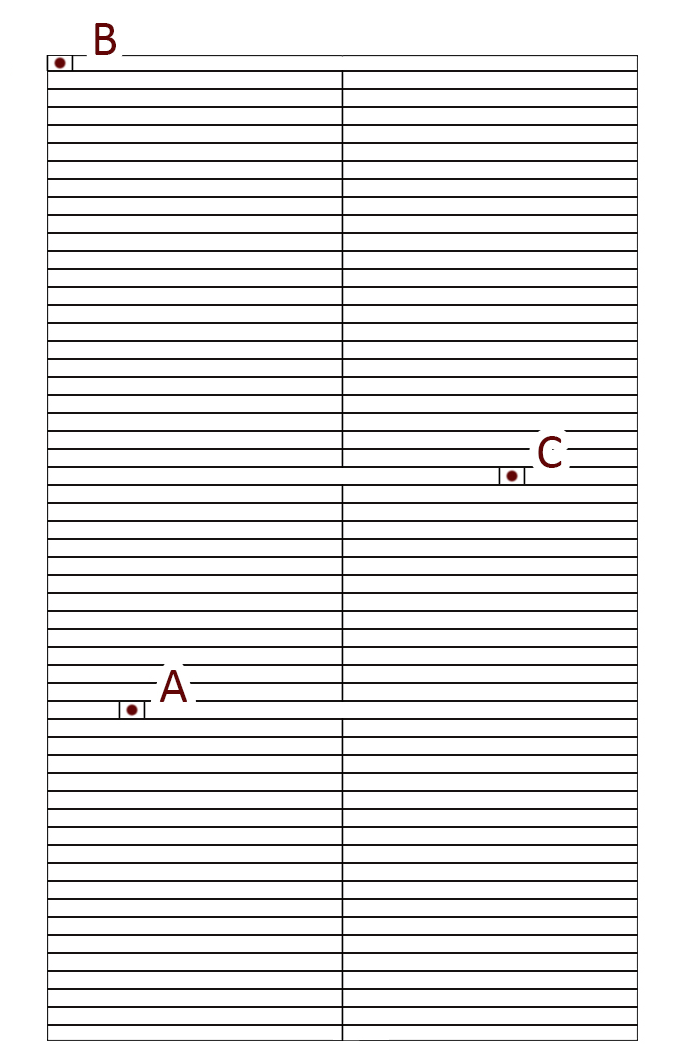
\includegraphics[height=0.8\textheight]{FIGURES/paso4}
		\end{center}
\end{frame}
%%%%%%%%%%%%%%%%%%%%%%%%%%%%%%%%%%%%%%%%%%%%%%%%%%%%%%%%%%%%%%

%%%%%%%%%%%%%%%%%%%%%%%%%%%%%%%%%%%%%%%%%%%%%%%%%%%%%%%%%%%%%%
\begin{frame}
    \frametitle{Algoritmo Constructivo}
    \block{Fase 2: Mejora}
    \endblock{}
		\begin{center}
    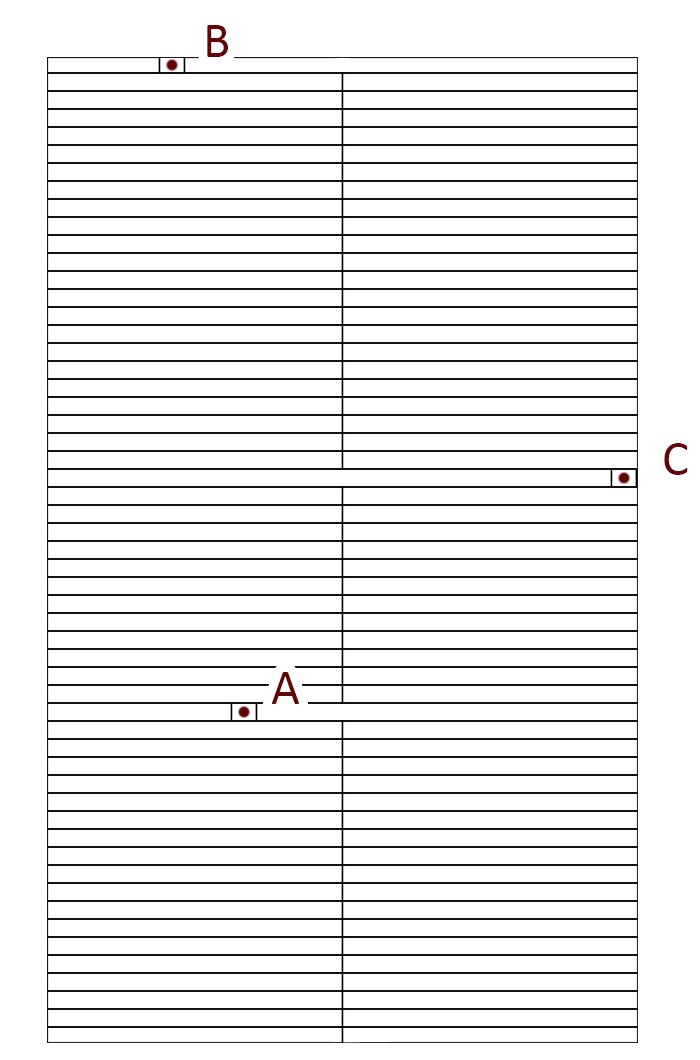
\includegraphics[height=0.8\textheight]{FIGURES/paso5}
		\end{center}
\end{frame}
%%%%%%%%%%%%%%%%%%%%%%%%%%%%%%%%%%%%%%%%%%%%%%%%%%%%%%%%%%%%%%

%%%%%%%%%%%%%%%%%%%%%%%%%%%%%%%%%%%%%%%%%%%%%%%%%%%%%%%%%%%%%%
\begin{frame}
    \frametitle{Obtención de objetos}
    \block{Problema - Colisión}
    \endblock{}
		\begin{center}
    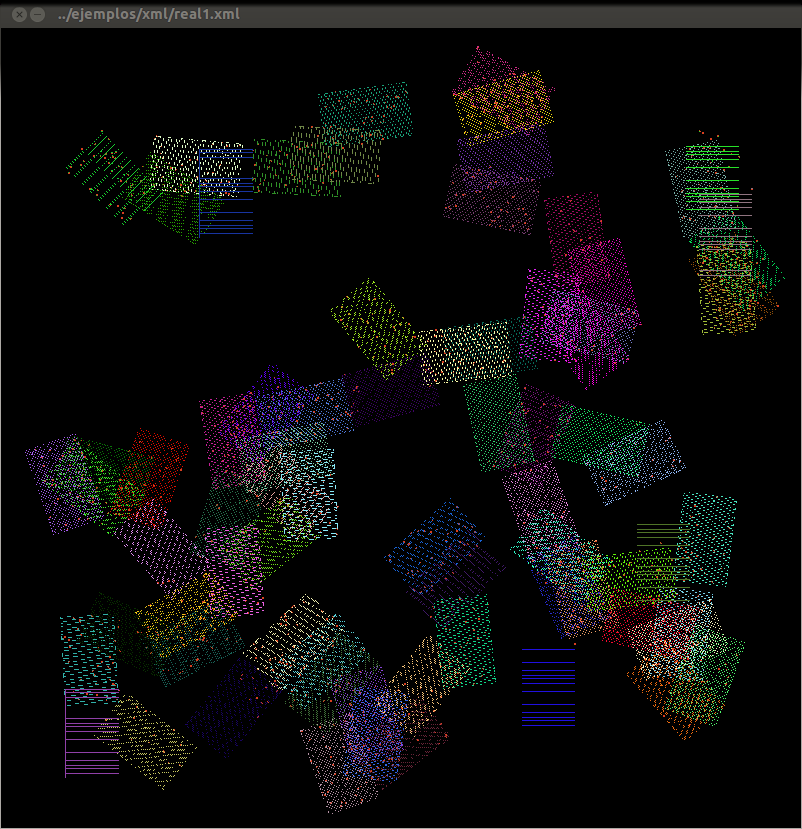
\includegraphics[height=0.8\textheight]{FIGURES/real1-out}
		\end{center}
\end{frame}
%%%%%%%%%%%%%%%%%%%%%%%%%%%%%%%%%%%%%%%%%%%%%%%%%%%%%%%%%%%%%%

%%%%%%%%%%%%%%%%%%%%%%%%%%%%%%%%%%%%%%%%%%%%%%%%%%%%%%%%%%%%%%
\begin{frame}
    \frametitle{Obtención de objetos}
    \block{Problema - Colisión}
    \endblock{}
		\begin{center}
    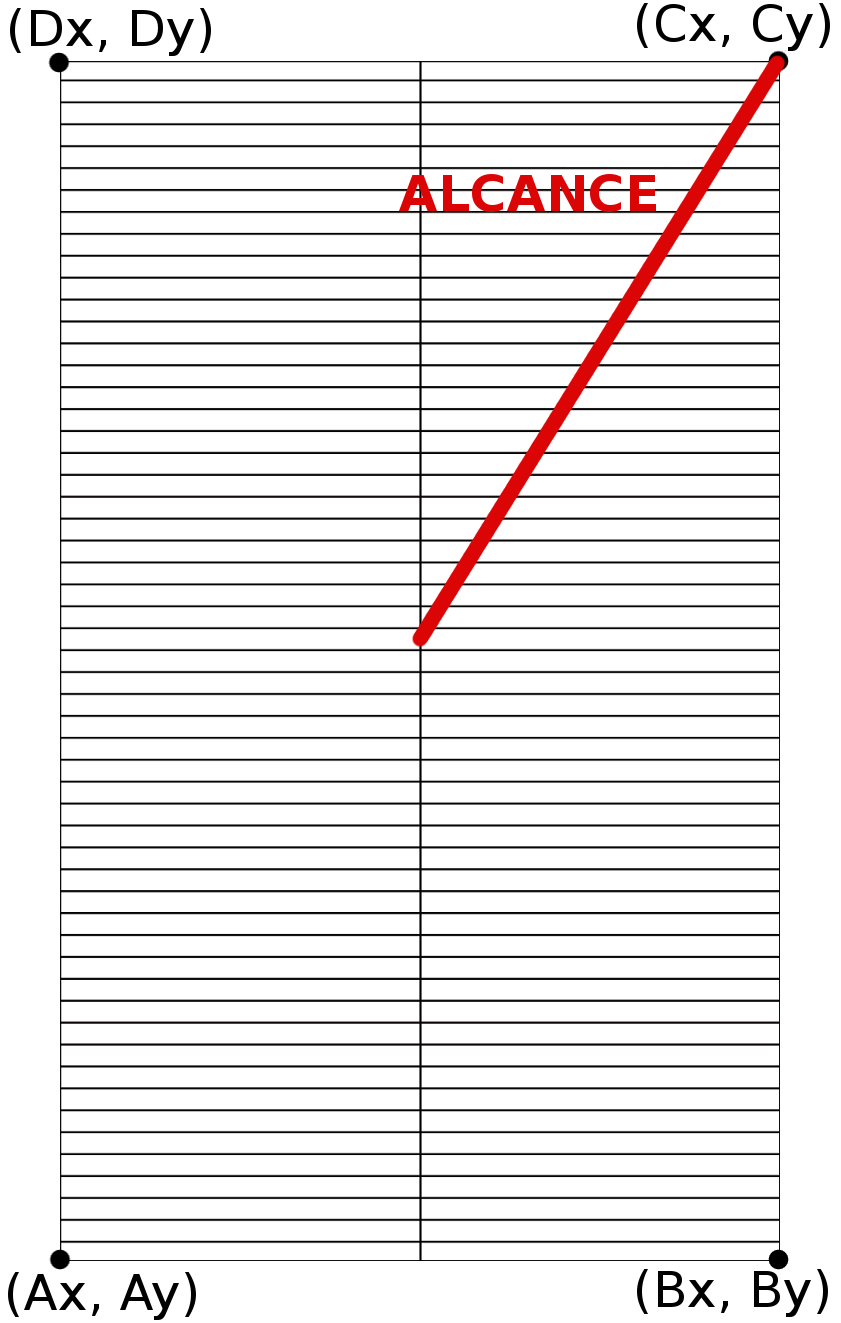
\includegraphics[height=0.8\textheight]{FIGURES/CSU-vertices}
		\end{center}
\end{frame}
%%%%%%%%%%%%%%%%%%%%%%%%%%%%%%%%%%%%%%%%%%%%%%%%%%%%%%%%%%%%%%






%%%%%%%%%%%%%%%%%%%% Code  %%%%%%%%%%%%%%%%%%%%%%%%%%%%%%%%%%%
\begin{frame}[fragile]
\frametitle{Reducción de colisiones}
%\block{}
%\endblock{}
\begin{lstlisting}[linewidth=\linewidth,
mathescape,numbers=none,basicstyle=\ttfamily\scriptsize]
$lista_{ini} =$ resultado
While(Mientras se mejore el resultado) {
    $lista_{fin} =$ los que no colisionan con ninguno.
    While(queden objetos por cubrir) {
        CSU $C \leftarrow$ primer apuntado $\in lista_{ini}$
        $subcto\_puntos = $ puntos de $C$
        Quitar $C$ de $lista_{ini}$
        While(queden CSUs $Q$ por mirar en $lista_{ini}$) {
            If($Q$ colisiona con $C$) {
                $subcto\_puntos += $ puntos de $Q$
                Quitar $Q$ de $lista_{ini}$
            }
        }
        If(colision innecesaria) {
            Obtener_nuevos_apuntados($subcto\_puntos$)
            If(consigue mejorar) 
              $lista_{ini} +=$ nuevos apuntado  
            else {
              Introducir en $lista_{ini}$ los que se quitaron
              Poner en $lista_{fin}$ el apuntado $C$
            }
        }
    }
    $lista_{ini} = lista_{fin}$
\end{lstlisting}
\end{frame}
%%%%%%%%%%%%%%%%%%%%%%%%%%%%%%%%%%%%%%%%%%%%%%%%%%%%%%%%%%%%%%


\section{\CSUO{}: Optimizando apuntados}
	  %\section{Aplicación}
%%%%%%%%%%%%%%%%%%%%%%%%%%%%%%%%%%%%%%%%%%%%%%%%%%%%%%%%%%%%%%
\begin{frame}[fragile]
    \frametitle{\CSUO{}}
    \block{Entrada/Salida}
    \endblock{}
\begin{lstlisting}[numbers=none]
./csuoptimizer [opciones] entrada.xml
\end{lstlisting}

\begin{lstlisting}[linewidth=\linewidth,numbers=none,language=XML,basicstyle=\ttfamily\scriptsize]
<Observables [widht=``Ancho_cielo'' height=``Alto_cielo'']>
    <Element id=``Identificador''>
        <X>PosX</X>
        <Y>PosY</Y>
        <Prioridad>[1..99]</Prioridad>
    </Element>
<!-- ...  -->
</Observables>
\end{lstlisting}
\end{frame}
%%%%%%%%%%%%%%%%%%%%%%%%%%%%%%%%%%%%%%%%%%%%%%%%%%%%%%%%%%%%%%

%%%%%%%%%%%%%%%%%%%% Code  %%%%%%%%%%%%%%%%%%%%%%%%%%%%%%%%%%%
\begin{frame}[fragile]
    \frametitle{\CSUO{}}
    \block{Entrada/Salida}
    \endblock{}
    \begin{lstlisting}[linewidth=\linewidth,numbers=none,language=XML,basicstyle=\ttfamily\footnotesize]
<Apuntado>
    <X>ValorX</X>
    <Y>ValorY</Y>
	  <PA>AnguloPosicion</PA>
	  <Configuracion>
		    <Barra>Posicion1</Barra>
		    <Barra>Posicion2</Barra>
            <!-- ...  -->
		    <Barra>Posicion54</Barra>
		    <Barra>Posicion55</Barra>
	  </Configuracion>
</Apuntado>
\end{lstlisting}
\end{frame}
%%%%%%%%%%%%%%%%%%%%%%%%%%%%%%%%%%%%%%%%%%%%%%%%%%%%%%%%%%%%%%

%%%%%%%%%%%%%%%%%%%% Code  %%%%%%%%%%%%%%%%%%%%%%%%%%%%%%%%%%%
%\begin{frame}[fragile]
%\frametitle{}
%\block{}
%\begin{lstlisting}[linewidth=\textwidth, numbers=none,basicstyle=\ttfamily\scriptsize]
%$ ./csuoptimizer --help
%
%Pointing optimizer program for Emir
%
%Usage: ./csuoptimizer [options] <input file>"
%
%Available options:
%--beams: activates beam switching (default is off).
%--dat: Changes output format to .dat (default is XML).
%--dbscan: Activates the use of DBScan cluster detection algorithm (default is off).
%--grasp: Uses the GRASP heuristic to enhance the results (default is off).
%--graphic: Activates graphic step by step execution for debugging purposes. It slows execution (default is off).
%--noborder: Avoids objects in the border of the bars.
%-NR X: X stands for the number of CSU rotations to perform when searching. Default is 20.
%--verbose: Generates the 'verbose.txt' text file containing information related to the program execution.
%
%The <input file> must be a XML file with this format:
%
%<Observables [widht=Ancho_cielo height=Alto_cielo]>
%		<Element id=\"Identificador\">
%				<x>PosX</x>
%				<y>PosY</y>
%				<Prioridad>[1..99]</Prioridad>
%		</Element>
% 				 ···
%</Observables>
%\end{lstlisting}
%\endblock{}
%\end{frame}
%%%%%%%%%%%%%%%%%%%%%%%%%%%%%%%%%%%%%%%%%%%%%%%%%%%%%%%%%%%%%%%

%%%%%%%%%%%%%%%%%%%%%%%%%%%%%%%%%%%%%%%%%%%%%%%%%%%%%%%%%%%%%%
\begin{frame}
    \frametitle{\CSUO{}}
    \block{Opciones}
    \begin{itemize}[<+->]
    \item Uso del DBScan (No)
    \item Elegir número de rotaciones (20)
    \item Elegir tipo de salida (XML)
    \item Tipo de barra (Normal)
    \end{itemize}
    \endblock{}
\end{frame}
%%%%%%%%%%%%%%%%%%%%%%%%%%%%%%%%%%%%%%%%%%%%%%%%%%%%%%%%%%%%%%

%%%%%%%%%%%%%%%%%%%%%%%%%%%%%%%%%%%%%%%%%%%%%%%%%%%%%%%%%%%%%%
\begin{frame}
    \frametitle{Tipos de barras}
    \block{Barras normales}
    \endblock{}
    
\includegraphics[width=0.4\linewidth]{FIGURES/BarraPunto1}
    \hspace{5mm}
    
\includegraphics[width=0.4\linewidth]{FIGURES/Bueno1}
\end{frame}
%%%%%%%%%%%%%%%%%%%%%%%%%%%%%%%%%%%%%%%%%%%%%%%%%%%%%%%%%%%%%%

%%%%%%%%%%%%%%%%%%%%%%%%%%%%%%%%%%%%%%%%%%%%%%%%%%%%%%%%%%%%%%
\begin{frame}
    \frametitle{Tipos de barras}
    \block{Barras sin bordes}
    \endblock{}
    
\includegraphics[width=0.4\linewidth]{FIGURES/BarraPunto2}
    \hspace{5mm}
    
\includegraphics[width=0.4\linewidth]{FIGURES/Bueno2}
\end{frame}
%%%%%%%%%%%%%%%%%%%%%%%%%%%%%%%%%%%%%%%%%%%%%%%%%%%%%%%%%%%%%%

%%%%%%%%%%%%%%%%%%%%%%%%%%%%%%%%%%%%%%%%%%%%%%%%%%%%%%%%%%%%%%
\begin{frame}
    \frametitle{Tipos de barras}
    \block{Barras con Beam Switching}
    \endblock{}
    
\includegraphics[width=0.4\linewidth]{FIGURES/BarraPunto3}
    \hspace{5mm}
    
\includegraphics[width=0.4\linewidth]{FIGURES/Bueno3}
\end{frame}
%%%%%%%%%%%%%%%%%%%%%%%%%%%%%%%%%%%%%%%%%%%%%%%%%%%%%%%%%%%%%%

%%%%%%%%%%%%%%%%%%%%%%%%%%%%%%%%%%%%%%%%%%%%%%%%%%%%%%%%%%%%%%
\begin{frame}
    \frametitle{Tipos de barras}
    \block{Barras con ambas opciones}
    \endblock{}
    
\includegraphics[width=0.4\linewidth]{FIGURES/BarraPunto4}
    \hspace{5mm}
    
\includegraphics[width=0.4\linewidth]{FIGURES/Bueno4}
\end{frame}
%%%%%%%%%%%%%%%%%%%%%%%%%%%%%%%%%%%%%%%%%%%%%%%%%%%%%%%%%%%%%%

\section{Resultados}
	  %\section{Resultados}

%%%%%%%%%%%%%%%%%%%%%%%%%%%%%%%%%%%%%%%%%%%%%%%%%%%%%%%%%%%%%%
\begin{frame}
    \frametitle{Resultados}
    \centering{
\includegraphics[width=0.8\linewidth]{FIGURES/logoAllegro}}
    \block{Allegro}
		\begin{itemize}
		\item Librería libre y de código abierto para la programación de videojuegos desarrollada en lenguaje C
		\item Funciones para gráficos, manipulación de imágenes, texto, sonidos, etc.
		\end{itemize}
    \endblock{}
\end{frame}
%%%%%%%%%%%%%%%%%%%%%%%%%%%%%%%%%%%%%%%%%%%%%%%%%%%%%%%%%%%%%%

%%%%%%%%%%%%%%%%%%%%%%%%%%%%%%%%%%%%%%%%%%%%%%%%%%%%%%%%%%%%%%
\begin{frame}
    \frametitle{Resultados}
    \block{Caso Real: cluster1.xml}
    \begin{itemize}
    \item 1398 objetos
    \item Distribución concéntrica
    \end{itemize}
    \endblock{}
		\begin{center}
    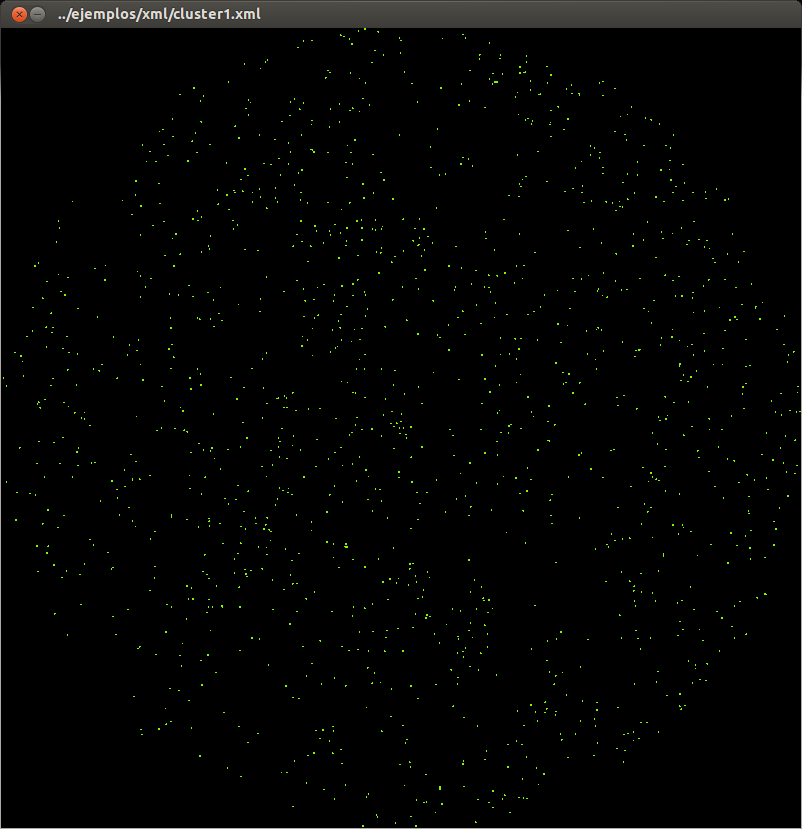
\includegraphics[height=0.55\textwidth]{FIGURES/cluster1-in}
		\end{center}
\end{frame}
%%%%%%%%%%%%%%%%%%%%%%%%%%%%%%%%%%%%%%%%%%%%%%%%%%%%%%%%%%%%%%

%%%%%%%%%%%%%%%%%%%%%%%%%%%%%%%%%%%%%%%%%%%%%%%%%%%%%%%%%%%%%%
\begin{frame}
    \frametitle{Resultados}
    \block{Caso Real: cluster1.xml}
    \begin{itemize}
    \item 1398 objetos
    \item Distribución concéntrica
    \end{itemize}
    \endblock{}
		\begin{center}
    \centering{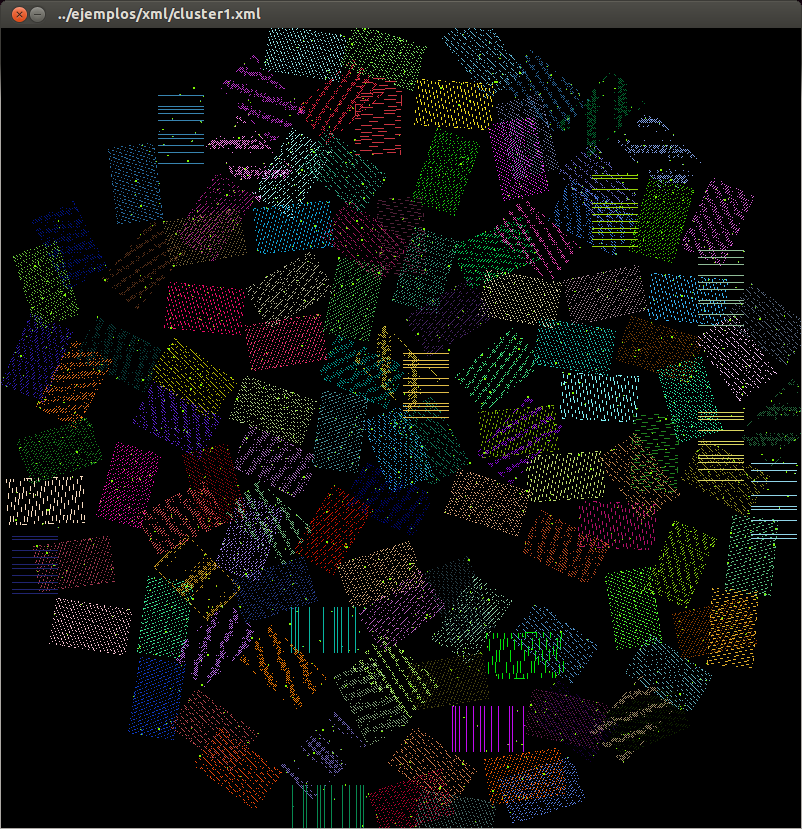
\includegraphics[width=0.55\textwidth]{FIGURES/cluster1-out}}
		\end{center}
\end{frame}
%%%%%%%%%%%%%%%%%%%%%%%%%%%%%%%%%%%%%%%%%%%%%%%%%%%%%%%%%%%%%%

%%%%%%%%%%%%%%%%%%%%%%%%%%%%%%%%%%%%%%%%%%%%%%%%%%%%%%%%%%%%%%
\begin{frame}
    \frametitle{Resultados}
    \block{Caso Real: cluster1.xml}
    {\ttfamily
\begin{tabular}{||l||c|c||}
\hline
\hline
RESULTADOS & Apuntados & Tiempo \\
\hline
\hline
Sin opciones & 123 & 45.04'' \\
\hline
Sin bordes &138 & 45.05'' \\
\hline
Beam Switching & 180 & 1' 29.35'' \\
\hline
Sin bordes + Beam S. & 218 & 1' 59.17'' \\
\hline
\hline
\end{tabular}}
    \endblock{}
\end{frame}
%%%%%%%%%%%%%%%%%%%%%%%%%%%%%%%%%%%%%%%%%%%%%%%%%%%%%%%%%%%%%%

%%%%%%%%%%%%%%%%%%%%%%%%%%%%%%%%%%%%%%%%%%%%%%%%%%%%%%%%%%%%%%
\begin{frame}
    \frametitle{Resultados}
    \block{Caso Real: cluster2.xml}
    \begin{itemize}
    \item 1842 objetos
    \item Distribución concéntrica
    \end{itemize}
    \endblock{}
		\begin{center}
    \centering{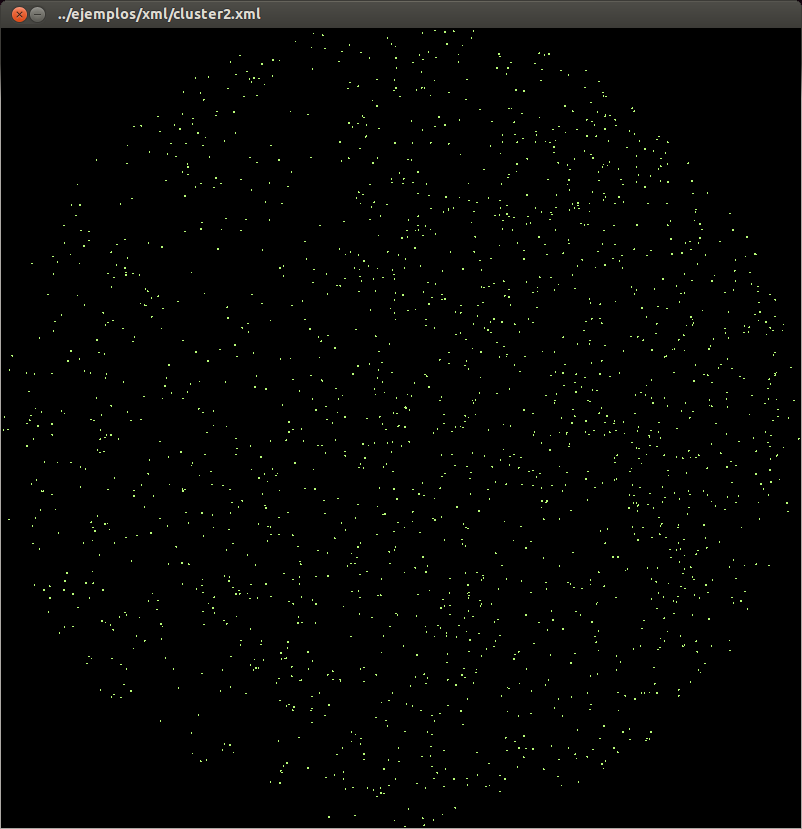
\includegraphics[height=0.55\textwidth]{FIGURES/cluster2-in}}
		\end{center}
\end{frame}
%%%%%%%%%%%%%%%%%%%%%%%%%%%%%%%%%%%%%%%%%%%%%%%%%%%%%%%%%%%%%%

%%%%%%%%%%%%%%%%%%%%%%%%%%%%%%%%%%%%%%%%%%%%%%%%%%%%%%%%%%%%%%
\begin{frame}
    \frametitle{Resultados}
    \block{Caso Real: cluster2.xml}
    \begin{itemize}
    \item 1842 objetos
    \item Distribución concéntrica
    \end{itemize}
    \endblock{}
		\begin{center}
    \centering{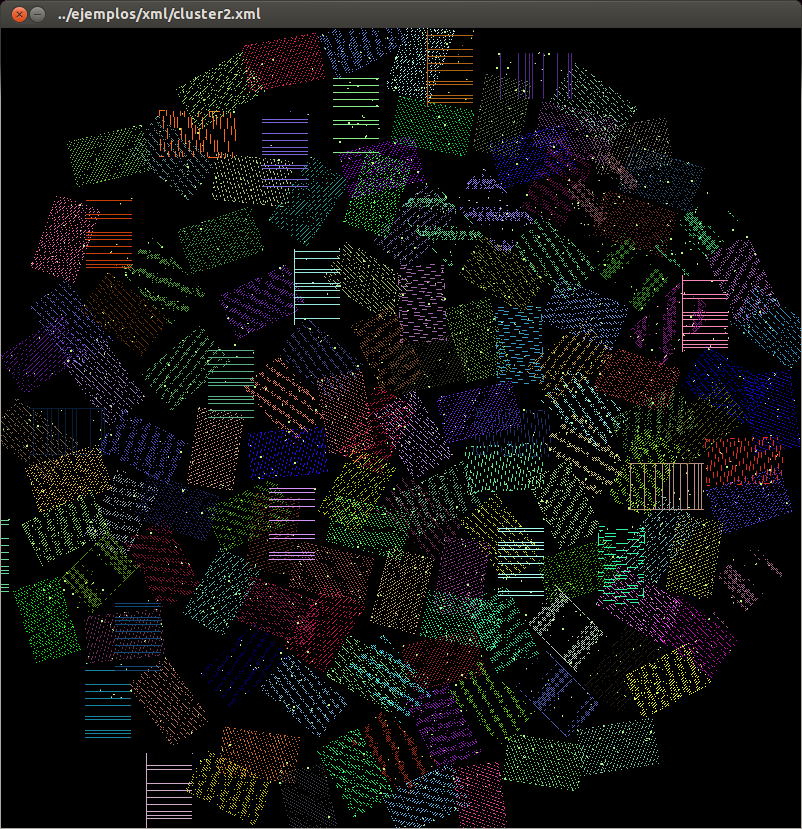
\includegraphics[width=0.55\textwidth]{FIGURES/cluster2-out}}
		\end{center}
\end{frame}
%%%%%%%%%%%%%%%%%%%%%%%%%%%%%%%%%%%%%%%%%%%%%%%%%%%%%%%%%%%%%%

%%%%%%%%%%%%%%%%%%%%%%%%%%%%%%%%%%%%%%%%%%%%%%%%%%%%%%%%%%%%%%
\begin{frame}
    \frametitle{Resultados}
    \block{Caso Real: cluster2.xml}
    {\ttfamily
\begin{tabular}{||l||c|c||}
\hline
\hline
RESULTADOS & Apuntados & Tiempo \\
\hline
\hline
Sin opciones & 138 & 1' 57.42'' \\
\hline
Sin bordes & 152& 2' 1.68'' \\
\hline
Beam Switching & 213 & 2' 19.05'' \\
\hline
Sin bordes + Beam S. & 263 & 4' 19.05'' \\
\hline
\hline
\end{tabular}}
    \endblock{}
\end{frame}
%%%%%%%%%%%%%%%%%%%%%%%%%%%%%%%%%%%%%%%%%%%%%%%%%%%%%%%%%%%%%%

%%%%%%%%%%%%%%%%%%%%%%%%%%%%%%%%%%%%%%%%%%%%%%%%%%%%%%%%%%%%%%
\begin{frame}
    \frametitle{Resultados}
    \block{Caso Real: cluster3.xml}
    \begin{itemize}
    \item 1074 objetos
    \item Distribución concéntrica
    \end{itemize}
    \endblock{}
		\begin{center}
    \centering{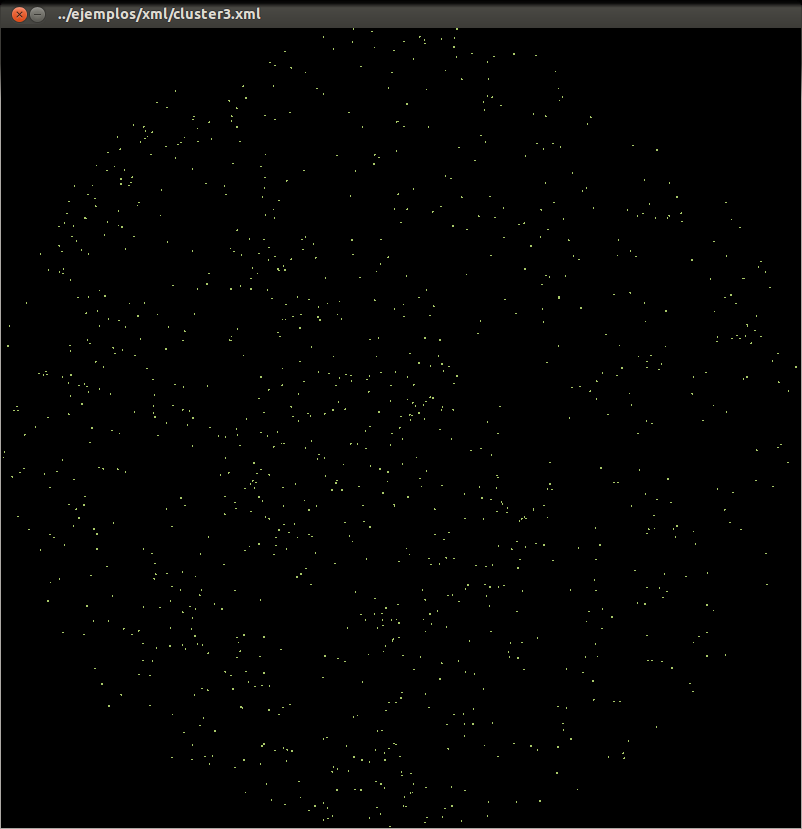
\includegraphics[height=0.55\textwidth]{FIGURES/cluster3-in}}
		\end{center}
\end{frame}
%%%%%%%%%%%%%%%%%%%%%%%%%%%%%%%%%%%%%%%%%%%%%%%%%%%%%%%%%%%%%%

%%%%%%%%%%%%%%%%%%%%%%%%%%%%%%%%%%%%%%%%%%%%%%%%%%%%%%%%%%%%%%
\begin{frame}
    \frametitle{Resultados}
    \block{Caso Real: cluster3.xml}
    \begin{itemize}
    \item 1074 objetos
    \item Distribución concéntrica
    \end{itemize}
    \endblock{}
		\begin{center}
    \centering{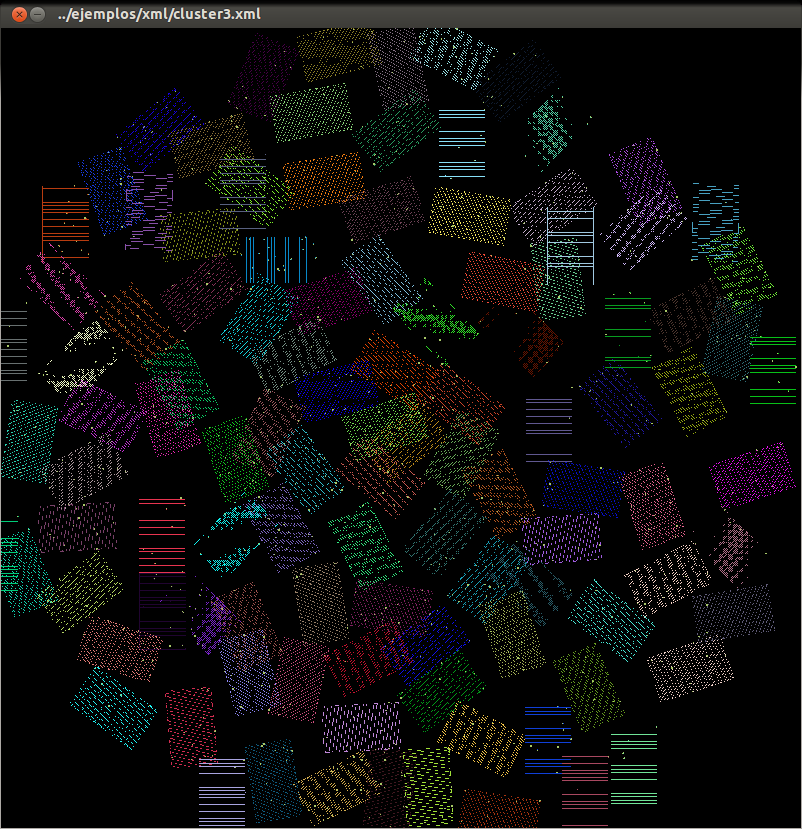
\includegraphics[width=0.55\textwidth]{FIGURES/cluster3-out}}
		\end{center}
\end{frame}
%%%%%%%%%%%%%%%%%%%%%%%%%%%%%%%%%%%%%%%%%%%%%%%%%%%%%%%%%%%%%%

%%%%%%%%%%%%%%%%%%%%%%%%%%%%%%%%%%%%%%%%%%%%%%%%%%%%%%%%%%%%%%
\begin{frame}
    \frametitle{Resultados}
    \block{Caso Real: cluster3.xml}
    {\ttfamily
\begin{tabular}{||l||c|c||}
\hline
\hline
RESULTADOS & Apuntados & Tiempo \\
\hline
\hline
Sin opciones & 109 & 31.09'' \\
\hline
Sin bordes & 117 & 38.57'' \\
\hline
Beam Switching & 153 & 1' 4.49'' \\
\hline
Sin bordes + Beam S. & 180 & 1' 16.68'' \\
\hline
\hline
\end{tabular}}
    \endblock{}
\end{frame}
%%%%%%%%%%%%%%%%%%%%%%%%%%%%%%%%%%%%%%%%%%%%%%%%%%%%%%%%%%%%%%

%%%%%%%%%%%%%%%%%%%%%%%%%%%%%%%%%%%%%%%%%%%%%%%%%%%%%%%%%%%%%%
\begin{frame}
    \frametitle{Resultados}
    \block{Caso Real: real2.xml}
    \begin{itemize}
    \item 297 objetos
    \item Distribución aleatoria dispersa
    \end{itemize}
    \endblock{}
		\begin{center}
    \centering{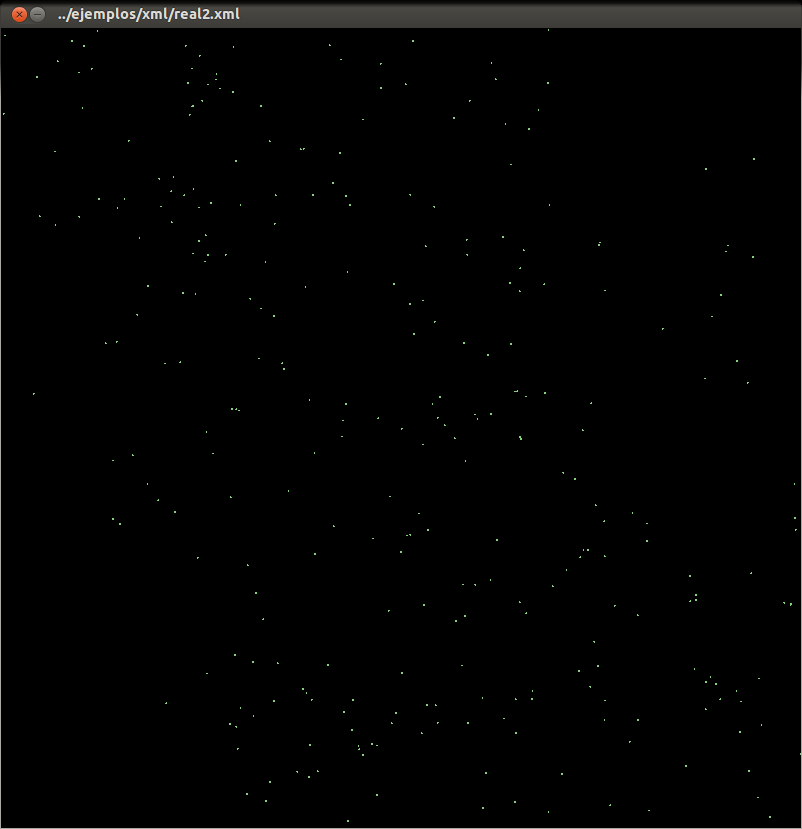
\includegraphics[height=0.55\textwidth]{FIGURES/real2-in}}
		\end{center}
\end{frame}
%%%%%%%%%%%%%%%%%%%%%%%%%%%%%%%%%%%%%%%%%%%%%%%%%%%%%%%%%%%%%%

%%%%%%%%%%%%%%%%%%%%%%%%%%%%%%%%%%%%%%%%%%%%%%%%%%%%%%%%%%%%%%
\begin{frame}
    \frametitle{Resultados}
    \block{Caso Real: real2.xml}
    \begin{itemize}
    \item 297 objetos
    \item Distribución aleatoria dispersa
    \end{itemize}
    \endblock{}
		\begin{center}
    \centering{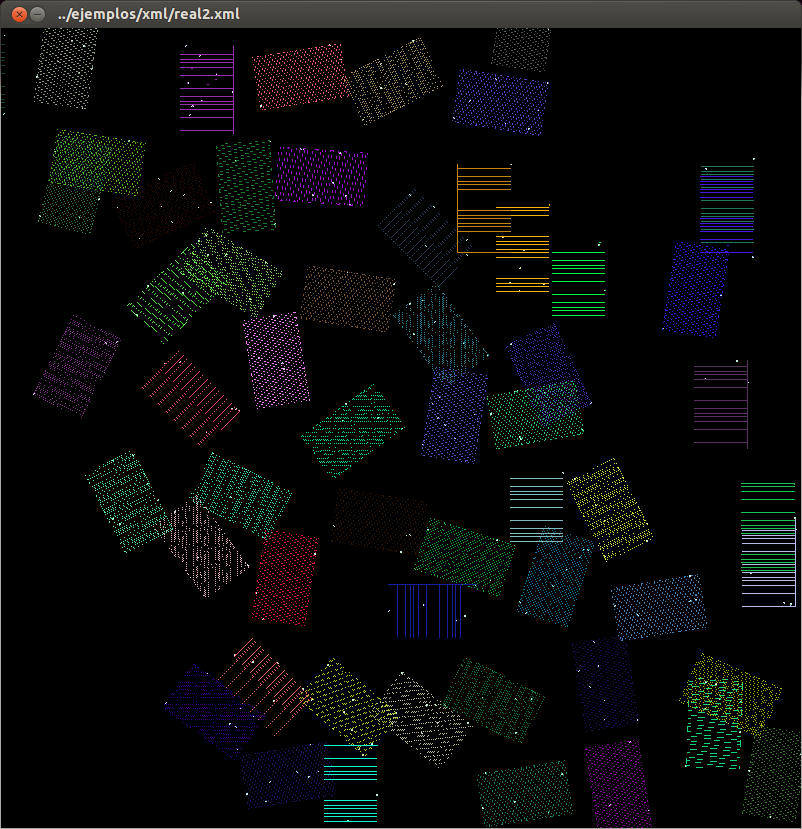
\includegraphics[width=0.55\textwidth]{FIGURES/real2-out}}
		\end{center}
\end{frame}
%%%%%%%%%%%%%%%%%%%%%%%%%%%%%%%%%%%%%%%%%%%%%%%%%%%%%%%%%%%%%%

%%%%%%%%%%%%%%%%%%%%%%%%%%%%%%%%%%%%%%%%%%%%%%%%%%%%%%%%%%%%%%
\begin{frame}
    \frametitle{Resultados}
    \block{Caso Real: real2.xml}
    {\ttfamily
\begin{tabular}{||l||c|c||}
\hline
\hline
RESULTADOS & Apuntados & Tiempo \\
\hline
\hline
Sin opciones & 57 & 3.85'' \\
\hline
Sin bordes & 56 & 3.91'' \\
\hline
Beam Switching & 70 & 6.24'' \\
\hline
Sin bordes + Beam S. & 79& 7.08'' \\
\hline
\hline
\end{tabular}}
    \endblock{}
\end{frame}
%%%%%%%%%%%%%%%%%%%%%%%%%%%%%%%%%%%%%%%%%%%%%%%%%%%%%%%%%%%%%%

%%%%%%%%%%%%%%%%%%%%%%%%%%%%%%%%%%%%%%%%%%%%%%%%%%%%%%%%%%%%%%
\begin{frame}
    \centerline{\LARGE{Volvamos a la prueba}}
\end{frame}
%%%%%%%%%%%%%%%%%%%%%%%%%%%%%%%%%%%%%%%%%%%%%%%%%%%%%%%%%%%%%%

\section{Conclusiones}
	  %\section{Conclusiones}

\begin{frame}
    \frametitle{Conclusiones}
    \block{Logros}
    \begin{itemize}[<+->]
    \item Investigación sobre posibles métodos para resolver el problema
\item Desarrollo de una aplicación plenamente operativa
\item Software documentado como punto de partida de desarrollos futuros
\item Documento técnico de la aplicación desarrollada
    \end{itemize}
    \endblock{}
\end{frame}


\begin{frame}
    \frametitle{Conclusiones}
    \block{Dificultades}
    \begin{itemize}[<+->]
\item La mejora de la calidad de las soluciones obtenidas
\item La reducción de los tiempos de ejecución
\item Estudio y selección de algoritmos para el problema planteado
\item Adaptarnos al lenguaje usual de los astrónomos
\item La comprensión de las características intrínsecas al problema
    \end{itemize}
    \endblock{}
\end{frame}

\begin{frame}
\frametitle{Trabajos futuros}
    \block{Posibles líneas de actuación}
    \begin{itemize}[<+->]
    \item Estudio de calidad de soluciones
    \item Margen de mejora en tiempos de respuesta
    \item Interfaz de usuario
    \end{itemize}
    \endblock{}
\end{frame}

%%%%%%%%%%%%%%%%%%%%%%%%%%%%%%%%%%%%%%%%%%%%%%%%%%%%%%%%%
\frame{
  \centerline{\LARGE{\textbf{Gracias por su atención}}}
}
\frame{\titlepage}
\end{document}
%%%%%%%%%%%%%%%%%%%%%%%%%%%%%%%%%%%%%%%%%%%
